% define document type (i.e., template. Here: A4 APA manuscript with 12pt font)
\documentclass[man, 12pt, a4paper, mask]{apa7}

% change margins (e.g., for margin comments):
%\usepackage{geometry}
% \geometry{
% a4paper,
% marginparwidth=30mm,
% right=50mm,
%}

% add packages
\usepackage[american]{babel}
\usepackage[utf8]{inputenc}
\usepackage{csquotes}
\usepackage{hyperref}
\usepackage[style=apa, sortcites=true, sorting=nyt, backend=biber, natbib=true, uniquename=false, uniquelist=false, useprefix=true]{biblatex}
\usepackage{authblk}
\usepackage{graphicx}
\usepackage{setspace,caption}
\usepackage{subcaption}
\usepackage{enumitem}
\usepackage{lipsum}
\usepackage{soul}
\usepackage{xcolor}
\usepackage{fourier}
\usepackage{stackengine}
\usepackage{scalerel}
\usepackage{fontawesome}
\usepackage[normalem]{ulem}
% \usepackage{longtable}
\usepackage{amsmath}
\usepackage{afterpage}
\usepackage{float}
\usepackage{array}
\usepackage{censor}

% add definition sections
\newtheorem{definition}{Definition}

% Select what to do with to-do notes: 
% \usepackage[disable]{todonotes} % notes not showed
% \usepackage[draft]{todonotes}   % notes showed

% make warning with red triangle
\newcommand\Warning[1][2ex]{%
  \renewcommand\stacktype{L}%
  \scaleto{\stackon[1.3pt]{\color{red}$\triangle$}{\tiny\bfseries !}}{#1}}%

% make question with red triangle
\newcommand\Question[1][2ex]{%
  \renewcommand\stacktype{L}%
  \scaleto{\stackon[1.3pt]{\color{red}$\triangle$}{\tiny\bfseries ?}}{#1}}%

% formatting links in the PDF file
\hypersetup{
pdfpagemode={UseOutlines},
bookmarksopen=true,
bookmarksopenlevel=0,
hypertexnames=false,
colorlinks   = true, %Colours links instead of ugly boxes
urlcolor     = blue, %Colour for external hyperlinks
linkcolor    = blue, %Colour of internal links
citecolor   = cyan, %Colour of citations
pdfstartview={FitV},
unicode,
breaklinks=true,
}

% language settings
\DeclareLanguageMapping{american}{american-apa}

% add reference library file
\addbibresource{references.bib}

% Title and header
\title{The Migration Experience: A Conceptual Framework and Systematic Review of Psychological Acculturation}
\shorttitle{Acculturation Experience Framework}

% Authors
\author[*,1,2]{Jannis Kreienkamp}
\author[1,2]{Laura F. Bringmann}
\author[1,2]{Raili F. Engler}
\author[1,2]{Peter de Jonge}
\author[1,2]{Kai Epstude}
\affiliation{\hfill}
\affil[1]{University of Groningen, Department of Psychology}
\affil[2]{Other affiliations still missing.}


\authornote{
   \addORCIDlink{* Jannis Kreienkamp}{0000-0002-1831-5604}\\
   \addORCIDlink{Laura F. Bringmann}{0000-0002-8091-9935}\\
   \addORCIDlink{Raili F. Engler}{0000-0002-4656-3672}\\
   \addORCIDlink{Peter de Jonge}{0000-0002-0866-6929}\\
   \addORCIDlink{Kai Epstude}{0000-0001-9817-3847}

We have no known conflict of interest to declare. The authors received no specific funding for this work. Source data and  software is available at \url{https://github.com/JannisCodes/acculturation-review} \citep{Kreienkamp2021b}. Protocols, materials, analysis data, and code are available at \url{https://doi.org/10.34894/U988DU} \citep{Kreienkamp2021a}. 

Correspondence concerning this article should be addressed to Jannis Kreienkamp, Department of Psychology, University of Groningen, Grote Kruisstraat 2/1, 9712 TS Groningen (The Netherlands).  E-mail: j.kreienkamp@rug.nl}

\leftheader{Kreienkamp}

% Abstract
\abstract{
One of the key challenges to researching psychological acculturation is an immense heterogeneity in theories and measures. These inconsistencies make it difficult to compare past literature on acculturation, hinder straight-forward measurement selections, and hamper the development of an overarching framework. To structure our understanding of the migration process, we propose to utilize the four basic elements of human experiences (wanting, feeling, thinking, and doing) as a conceptual framework. We use this framework to build a theory-driven literature synthesis of past theoretical (final \textit{N} = 92), methodological (final \textit{N} = 233) and empirical literature (final \textit{N} = 530). We find that especially empirical works have understudied the more internal aspects of acculturation (motivations and feelings) and have often fallen short of capturing all four aspects of the migration experience. We also show differences between publication fields and discuss how the framework can aid transparent and functional theories, studies, and interventions going forward.

\noindent\textbf{Public significance statement}: This systematic review indicates that the concept of psychological acculturation can be structured in terms of affect (e.g., feeling at home), behavior (e.g., language use), cognition (e.g., ethnic identification), and desire (e.g., independence wish). We find that although theoretical literature focuses substantially on emotional and motivational as well as dynamic conceptualizations, in empirical studies this is often not the case. This shows a crucial disconnect between theory and practice.
}

\keywords{Psychological Acculturation, Experience, Framework, Systematic Review}


% set indentation size
\setlength\parindent{1.27cm}

% Start of the main document:
\begin{document}

% add title information (incl. title page and abstract)
\maketitle

% **CHEAT SHEET / LEGEND**
%
% Comments:
% '%' starts a comment in LaTeX (not printed)
% '\todo[inline]{} makes orange boxes in PDF
% '\marginpar{}' notes in margins
% '\footnote{}' footnote
% '\Warning' important note indicator in PDF (triangle with exclamation mark)
% '\Question' question note indicator in PDF (triangle with question mark)
%
% Citation (with Natbib citation style):
% '\citep[e.g.][p. 15]{CitationKey}' citation in parentheses "(e.g., Berry, 2003, p. 15)"
% '\citet{CitationKey}' citation in text "Berry (2003)"
% '\citealt' and '\citealp' alternate citation without parentheses
% '\citeauthor' and '\citeyear' only year or author
% 
% Headings:
% '\part{}' and '\chapter{}' only relevant for multi-part or multi-chapter documents
% '\section{}' heading level 1
% '\subsection{}' heading level 2
% '\subsubsection{}' heading level 3
% '\paragraph{}' heading level 4
% '\subparagraph{}' heading level 5
%
% formatting:
% '\textbf{}' text bold font
% '\textit{}' text italic font
% '\underline{}' text underline
% '\sout{}' text strike out
% '\textsc{}' text small caps
% '\vspace{1em}' add vertical space
% '\hspace{1em}' add horizontal space
% '\\' new line (i.e., line break)
% '\pagebreak' start new page (i.e., page break)
% '\noindent' do not indent current line (e.g., current paragraph)
% 'begin{center}...end{center}' center text or object
%
% Math mode:
% '$\alpha = .8$' mathematical equation inline
% '$$\hat{y} = b_0 + b_1x$$' mathematical equation in its own line
% '\begin{equation}...\end{equation}' multi-line equation
% '\approx' approximate symbol
% '\neq' not equal
% '\bar' mean bar over letter
% '\pm' plus minus sign 
% '^{}' superscript
% '_{}' subscript
% '\fraq{numerator}{denominator}' fraction
% '\sqrt[n]{}' square root
% '\sum_{k=1}^n' sum for 1 through n
%
% Insert things from elsewhere:
% '\input{filename}' inputs the raw (tex) file as a command (e.g., tables and R-Markdown imports)
% '\include{filename}' includes section on new page (incl. possible auxiliary info)
% '\includegraphics[settings]{filename}' add a figure or graph
% '\caption{}' adds a caption to a table or figure
% '\label{}' labels sections, tables, figures, etc. so that they can be referred to.
% '\ref{}' refer to a labelled sections, tables, figures, etc.
% '\begin{enumerate}...\end{enumerate}' numbered list
% '\begin{itemize}...\end{itemize}' bullet-ed list
% '\item' item in list section 
%
% Symbols:
% '\&' and sign
% '\%' percent sign
% '\_' three dotes
% '\#' hash symbol
% ------------------------------------------------------------------


% Relevance
% Long discussed and relevant to society
The question of how people change when they get into continuous first-hand contact with other cultures is probably as old as the history of human migration. Answering this question remains an important issue for many societies around the world. 
Over the past 80 years, researchers of the psychological sciences have proposed hundreds of models and measurements for this phenomenon of "psychological acculturation" \citep[][]{Rudmin2003a}. Yet, despite enormous theoretical and empirical advances, it remains unclear what psychological acculturation exactly entails and a conceptual framework allowing for a synthesis of the past literature on psychological acculturation is still missing \citep{Birman2014c}.

% Problem - Illustration: Past Theory Use
We find an illustration of this challenging heterogeneity in the use of prominent theories of psychological acculturation. One prominent approach has been to conceptualize psychological acculturation as a two-dimensional set of orientations towards the heritage- and the dominant culture --- Berry's (\citeyear{Berry1980, Berry1997b, Berry2005}) now famous `acculturation orientations'. However, over the past 40 years, Berry himself has used a variety of attitudes (i.e., preferences) and behaviors (i.e., actual activities) to describe what these orientations should entail \citep{Berry2005}. And a broader review of the theory found that other researchers had conceptualized and measured `acculturation orientations' with even more diverse aspects. Conceptualizations had, for example, included attitudes, attachments, goals, identifications, or choices and uses of cultural elements \citep[e.g., language, food, or dresses. See,][]{Rudmin2003a}. We see a similar pattern with conceptualizations of psychological acculturation as a `psychological and socio-cultural adaptation' process. Here, cultural adaptation has, for example, included aspects such as life satisfaction and well-being, as well as cultural skills, and work performance \citep{Searle1990, Ward2001, Berry2003}.
Measurements of psychological acculturation are, thus, inconsistent across studies and it remains unclear what aspects the concept exactly entails, and how these aspects are organized.

% Problem - Consequences
% Theory and Application; Past and Future
This heterogeneity of aspects presents fundamental challenges to researchers, practitioners, and policy-makers in the field. Looking back at past theories and measures, different conceptualizations might lead to different results \citep{Snauwaert2003} and the diversities of included or excluded concepts makes it virtually impossible to compare different studies --- which makes it difficult to integrate them quantitatively or qualitatively \citep{Taft1981}.
And looking forward, it remains difficult to select acculturation elements and develop new theories and measurements. A coherent conceptual framework would be necessary to make informed and transparent choices on which aspects are (ir)relevant to a given research question and how they relate to one another.
Given these challenges, some have even suggested that psychological acculturation should not be measured until common terminologies and frameworks are available \citep{Escobar2000}.

% Aim - General
% Therefore we suggest a conceptual framework
The aim of this paper is, therefore, to offer a descriptive conceptual framework to analyze, measure, and understand the concept of psychological acculturation. Such a framework has a different objective than previous efforts which have catalogued literature on acculturation \citep[e.g.,][]{Castels2003}, built multidimensional measures of integration \citep[e.g.,][]{Harder2018}, normative frameworks \citep[e.g.,][]{Ager2008a}, or theories of acculturation \citep[e.g.,][]{Berry2005}. Rather than offering a new measurement, definition, or theory, we aim to build a framework to assess and compare these conceptual elements. 

% Aim - Specific
% We do this by using ABCD
To build a framework that would comprehensively structure the concept of psychological acculturation across a wide range of contexts, we propose to utilize the basic elements of human experiences.
Building on discussions with experts in the field and past reviews, we propose that the psychological acculturation experience can be understood in terms of affects, behaviors, cognitions, and desires. Psychological acculturation in this framework might, for example, be understood or measured in terms of behavioral acculturation, such as language use, or voting; cognitive acculturation, such as ethnic identification, or cultural values endorsement; affective acculturation, such as feeling at home, or loneliness; motivational acculturation, such as the satisfaction of competence or independence needs; or as a combination of any or all of these aspects (also see Table \ref{tab:AspectExamples} for a range of example concepts). 

% Structure of Paper
In the following sections, we will develop this framework in more detail and will then apply it to a systematic review of the past theoretical, methodological, empirical literature on acculturation.

\begin{table}%[hbt]
\caption{Examples of Coding Levels for the Experience Framework of Psychological Acculturation.}
\label{tab:AspectExamples} 
\begin{tabular}{>{\raggedright\arraybackslash}p{0.15\linewidth} 
>{\raggedright\arraybackslash}p{0.20\linewidth} 
>{\raggedright\arraybackslash}p{0.35\linewidth} 
>{\raggedright\arraybackslash}p{0.25\linewidth}}
\hline 
Aspect & Construct & Concept & Operationalization \\ 
\hline \\ [-0.5em]
Affect & 
Moods \linebreak Emotions \linebreak Feelings \linebreak & 
Loneliness \linebreak Feeling at home \linebreak Satisfaction with life \linebreak Pride \linebreak Comfortableness \linebreak Joy \linebreak Ease \linebreak Well-being \linebreak Worry \linebreak Trust \linebreak & 
"I feel ..." \linebreak "My mood ...." \linebreak "I enjoy ..." \linebreak \\

Behavior & 
Activities \linebreak Habits \linebreak Mannerisms \linebreak & 
Language use \linebreak Civic participation (voting, ...) \linebreak Performance (work, ...) \linebreak Media consumption \linebreak Educational achievement \linebreak Peer contacts \linebreak Food consumption \linebreak Cultural habits (holidays, ...) \linebreak Delinquency \linebreak Marriage \linebreak & 
"I do ..." \linebreak "I speak ..." \linebreak "I meet ..." \linebreak \\ 

Cognition & 
Knowledge \linebreak  Memories \linebreak Evaluations \linebreak & 
Ethnic identification \linebreak Cultural values \linebreak Acculturation orientation \linebreak Preferences (food, friends, ...) \linebreak Knowledge \linebreak Importance ratings \linebreak Inner thought language \linebreak Perceived obligations \linebreak Beliefs \linebreak Stereotypes \linebreak & 
"I prefer ..." \linebreak "I think ..." \linebreak "I identify as ..." \linebreak \\ 

Desire & 
Needs \linebreak Goals \linebreak Wants \linebreak & 
Competence \linebreak Independence \linebreak Self-coherence \linebreak Belonging \linebreak Achievement \linebreak Justice \linebreak Growth \linebreak Respect \linebreak Acceptance \linebreak Identity continuity \linebreak & 
"I want ...",\linebreak "I would like to ..." \linebreak "I need ..." \linebreak \\ 

\hline \\ [-0.75em]
\multicolumn{4}{p{\linewidth}}{\footnotesize \textit{Note.} Some of the concepts might include multiple experience aspects depending on the context.}

\end{tabular}
\end{table}


\section{Framework Development} 
This framework was developed based on collaborations with resettlement organizations and migrant citizens as well as based on past reviews and theoretical developments within the field. A focus group discussion with key societal stakeholders inspired this undertaking and laid the groundwork for the development of an experience framework of psychological acculturation\footnote{For the focus group discussion we reached out to societal stakeholders of the acculturation process to gather information on key acculturation aspects in the lived realities out in the field. These experience reports formed the earliest foundation of our framework aspects. The focus group consisted of voluntary migrants, refugees, teachers, language- and integration coaches, volunteers and staff of a regional refugee resettlement agency as well as a representative of the local government. The 12 carefully selected and invited participants joined a 120 minutes round-table focus group discussion on the concept of acculturation. With informed consent by the participants, the discussion was audio recorded, transcribed, and later coded in three coding cycles of (1) initial In Vivo coding using the participants own words, (2) open coding inductively identifying common topics and elements, as well as (3) a content analysis using focused coding to summarize the overarching themes, which included the experience elements discussed here.}. Yet, at the same time, the framework also grew out of a strong theoretical tradition in the field and arguably brings together many of the past advances in capturing psychological acculturation. We will first briefly address the notion of using a phenomenological approach for psychological acculturation and will then introduce each of the experience aspects before we apply the framework in a systematic literature review.

% Experience Structure
There is a converging theoretical consensus that human experiences can fundamentally be understood as a set of needs, feelings, thoughts, and behaviors \citep[sometimes referred to as the ABCs or ABCDs of psychology: affect, behavior, cognition, desire; e.g.,][]{Cottam2010, Hogg2005, Jhangiani2014}.\footnote{It should also be noted that ABC(D) frameworks have been used effectively to structure theories and models across a wide variety of fields --- including research on attitudes \citep{Breckler1984} and ambivalence \citep{VanHarreveld2015}, the self \citep{Cote2009} and self-regulation \citep{Ben-Eliyahu2015}, the big five personality traits \citep{Wilt2016}, suicidality \citep{Harris2015} and in clinical interventions \citep{Eifert1989}. Interestingly, the affect, behavior, and cognition structure has even found application in the development of human-like machines \citep{Guo2020}.} Following the premise that any human experience can be conceptualized within these four basic elements, we believe that an ABCD framework of psychological acculturation could offer a comprehensive and theory-driven framework to structure and analyze the concept of psychological acculturation. Importantly, affect, behavior, cognition, and desire are ideally suited to structure the concept of psychological acculturation in particular, because all four aspects (1) are influenced by culture, (2) are relevant in the interactions between cultures, and (3) are fundamental to the concept of adaptation.

% Culture
% Definition: culture as external social expectations focused on our "manners of acting, thinking and feeling, which are invested with a coercive power by virtue of which they exercise control over him" \citep[][p. 52; on social facts]{Durkheim1982, Gilbert1989}.
Cultures are often defined as external social expectations focused on our "manners of acting, thinking and feeling, which are invested with a coercive power by virtue of which they exercise control over him" \citep[][p. 52; on social facts]{Durkheim1982, Gilbert1989}. In such an understanding, cultures, for example, define expected patterns of behavior (e.g., dress or communication styles), cognition (e.g., sense of race-, class-, gender-, and sexual identities), emotions (e.g., expressions of emotions), and motivations (e.g., virtues and duties)\footnote{For a discussion of culture and behavior see for example \citet[][]{Legare2019, Whiting1980}, for cognitions see for example \citet[][]{Gelfand2011, Nisbett2002}, for emotions see for example \citet[][]{Holodynski2012, Boiger2018}, and desires see for example \citet[][]{McInerney2016, Morling2017}.}. The study of affect, behavior, cognition, and desire is, thus, well-aligned with the experience of culture in acculturation.

% Interaction
Additionally, affect, behavior, cognition and desire are also closely related to inter-group and inter-cultural contacts --- which is an essential condition for acculturation to occur. How and why people get into behavioral contact with people from other backgrounds has, for example, been linked to group-specific needs, and desires, such as power and acceptance \citep[e.g.,][]{Hassler2021, Shnabel2008a}. Similarly, outcomes of these interactions are often governed by inter-group cognitions, such as perceptions of threat or shared identities \citep[e.g.,][]{Dovidio2017, Stephan2000a} and inter-group emotions, including pride, or anxiety \citep[e.g.,][]{Iyer2008, Stephan1992}. Affect, behavior, cognition, and desire are, thus, also at the very heart of contacts between cultural groups.

% Adaptation
And lastly, affect, behavior, cognition, and desire have all been highlighted in the conceptualization of human functioning and adaptation --- a core outcome for many acculturation researchers \citep[e.g., see][]{Berry2006a,Searle1990,Ward2001,Maertz2016}. Adaptation in such an understanding can include, behavioral adaptions, such as building skills and competences \citep[e.g.,][]{Bevan1965}, cognitive adaptation, including self-image restorations and dissonance reductions \citep[e.g.,][]{Czajkowska2017}, emotional adaptions, such as dealing with feelings of culture shock and homesickness \citep[e.g.,][]{Smith1990, VanTilburg1996}, as well as desire adaptations, such as regulations of status and affection needs \citep[e.g.,][]{Steverink2006}. In sum, affects, behaviors, cognitions, and desires not only form the fundamental aspects of human experiences but also have a deep connection to culture, cultural contacts, and psychological adaptation --- which are essential to the idea and definition of psychological acculturation.

% ABC in Theoretical Traditions
Interestingly, the ABC structure is not entirely foreign to the field of acculturation. Ward and colleagues \citep{Ward2001, Masgoret2006, Ward2019} have previously pointed out that theoretical perspectives on acculturation tend to focus on affect, behavior, or cognition (forming the ABCs of acculturation). Within the affective tradition Ward situates the stress and coping literature, behavioral traditions are the cultural learning theories, and social identification theories form the cognitive theories. \citet{Sam2006b} and others have even noted that such a perspective might be useful in structuring the core components of psychological acculturation. 
Following Sam's (\citeyear{Sam2006b}) suggestion, we propose that, once we include desires (i.e., motivational literature), an expanded ABCD structure would not only summarize theoretical traditions but would offer a universal and theory-based framework to the concept of psychological acculturation because it comprehensively structures the fundamental aspects of the human experience.

In the next sections we will discuss how each of the aspects emerged out of the focus group discussion as well as conceptual developments within the field. 

\subsection{Behavior}
\begin{displayquote}
    Maria:\\
    {[...]} \textit{while, of course, you integrate best when you go to work.}
    
    Moderator:\\
    \textit{Why is that exactly?}
    
    Maria:\\
    {[...]} \textit{Because there you have daily contacts with locals.}
\end{displayquote}

% Focus Group Discussion
Behaviors --- that is actions and mannerisms --- were one of the major themes within the focus group discussion because they were perceived as particularly visible and subjected to clear expectations by the dominant group. The discussants especially focused on social behaviors (such as language learning and contacts outside the home) as interactive and reciprocal elements of psychological acculturation because they enable connections to the culture and being an active member of society.

% Past literature
Given the overt nature of behaviors and their interconnectedness with culture, behaviors have also been a prominent aspect of the acculturation literature. Ward and colleagues (\citeyear{Ward2019}) in their review have identified cultural learning theories as one key literature tradition that has focused on behavioral aspects of acculturation. They relate these learning theories to the acquisition of effective skills and competences as the behavioral operationalizations \citep[including, verbal and non-verbal communication skills][]{Ward2001}. Other examples of behavioral conceptualizations of acculturation (beyond Ward's focus), include civic participation \citep[e.g., voting;][]{Lessard-Phillips2020}, inter-ethnic marriage \citep[e.g.,][]{Song2009}, and media consumption \citep[e.g.,][]{Shoemaker1985}. 

\subsection{Cognition}
\begin{displayquote}
    Yahya:\\
    {[...]} \textit{Once I started my education, I felt part of society.} {[...]} \textit{That was not the case when I was learning Dutch at the university, at the language school, or at other places before. Only later when I was at school, ... I feel: Okay, now I feel I am really in the Netherlands.}
    
    Joop:\\
    \textit{Why did you not have that at the language school?}
    
    Yahya:\\
    \textit{Because I was only a refugee.}
\end{displayquote}

% Focus group discussion
Cognitive aspects, which commonly entail the thinking processes of the human experience, were also highlighted in the focus group discussion because they pertain to many navigational issues in society. Language-, social- and communication norms and learning about more formal social systems, values, and social rules were examples of how cognitive changes related to bridging social gaps. A second major topic discussed was the role of identity development. The newcomers pointed to both a break in identity (the struggle of defining oneself in the new environment) as well as the struggle of dealing with a singular (migrant or refugee) identity label and the process of developing a more complex identity narrative towards others.

% Past literature
Given the pertinent connection between cultures and cognitive processes, it might come as little surprise that cognitions have also played a major role in the acculturation literature. Within the cognitive tradition, Ward and colleagues (\citeyear{Ward2001, Ward2019}) have identified ethnic identity and group perception theories, with a particular focus on Berry's (\citeyear{Berry1997b}) acculturation attitudes. Beyond the theories identified by Ward, the acculturation literature has recently also focused on several other cognitive conceptualizations of psychological acculturation, including cultural values \citep[e.g.,][]{Marin2003} and stereotypes \citep[e.g.,][]{Stanciu2018}. 

\subsection{Affect}
\begin{displayquote}
    Fariq:\\
    {[...]} \textit{But for me the language is very very difficult. And then you think people are not open. And you don't understand because your language isn't that good. And then I maybe don't feel welcomed when I have questions or want to approach them.}
\end{displayquote}

Affect --- the human capacity to feel \citep[including emotions and moods;][]{FeldmanBarrett2007} --- was a prominent theme in the focus group discussion because it foregrounded the importance of the subjective experience as acculturation. Instead of focusing on purely behavioral outcome conceptualizations (e.g., housing, job, education), the group highlighted the importance of considering the affective acculturation experience (e.g., feeling at home, feeling accepted). As an example, when asked why having a job is important to acculturation, newcomers and supporters pointed to a feeling of usefulness and being part of society. 

% Past literature
But affect and emotion have also been discussed within the psychological acculturation literature. \citet{Ward2001} in her review of the acculturation traditions, describes the stress and coping literature --- especially Berry's concept of acculturation stress \citep{Berry1997b} --- as the affect component of acculturation. In this tradition, the main constructs that constitute the affective dimension are the psychological and emotional well-being as part of the psychological adaptation process \citep[including, for example, life satisfaction and depression;][]{Ward2019}. However, beyond the theoretical stress literature tradition, there are also more immediate models and measurements of emotional acculturation. There is, for example, a relatively young tradition of 'emotional acculturation' as a distinct concept in which acculturation is understood as the similarity in emotional patterns \citep[see][for a review]{DeLeersnyder2017}. But also individual emotions, such as 'feeling accepted' \citep{Jasini2018}, or 'pride' \citep{Suinn1995} have received attention as discrete conceptualizations of acculturation. 

\subsection{Desire}
\begin{displayquote}
    Yahya:\\
    {[...]} \textit{Yes, they [parents] have control like a boss or a god. And I still had that in Syria but it kind of stopped, ... because I am not gonna be a kind of a slave to my family, ... because I want freedom for myself.}
\end{displayquote}

% Focus group discussion
Desires --- the motivational forces of the human experience --- were likely discussed most interestingly during the focus group discussion. The (lack of) motivation to interact with the new culture and its members was one key discussion point but motives for actions and psychological needs of the migrants were also discussed as more impalpable properties of other acculturation aspects (e.g., the need for acceptance during interactions). Yet, importantly the motivational aspect also highlighted the functional essence of individual acculturation. The needs for interactions, to be understood, for purpose, and for identity continuity were discussed as not necessarily expected by the dominant group but as intrinsic and fundamental to the health and functioning of the newcomers during the acculturation process.

% Past literature
Yet, despite these deep connections, few of the past reviews have examined motivation as a distinct aspect of psychological acculturation within the literature or the concept. However, outside of reviews, needs and wants have been discussed more frequently as a conceptual aspect of psychological acculturation --- with more researchers looking at the reasons for migration \citep{Sandu2018}, as well as the motivations of acculturation orientations \citep{Recker2017a}, acculturation behavior \citep{Reece2000}, and psychological adaptation \citep{Safdar2003}. 

\subsection{The Lived Acculturation Experience}
% Experience elements and lived experience
While we have introduced the four experience aspects as distinct elements, it is important to note that both in theory and in practice affect, behavior, cognition, and desire are not experienced as distinct entities. This was highlighted during the focus group discussion but is also reflected in theories on the aspects. As an example, most emotions have a cognitive component just as most cognitions have an emotional value. Similarly, motivation is commonly conceived as having both emotional (e.g., desire) and cognitive (e.g., goals) aspects, both of which are often directed towards behaviors (i.e., conation). Muddying the waters further is the difficulty that many operationalizations (and empirical measures) of psychological acculturation also include multiple aspects. Concepts such as satisfaction or distress, which are common measures of acculturation, famously include emotional and cognitive components.  Yet, despite the interdependence of aspects in theories and lived experience, the four elements can consistently be identified within experiences and concepts --- they remain qualitatively different aspects of the experience. And as such, they offer a pragmatic lens to structure the psychological acculturation concept \citep{Kuhn1962}. Differentiating the four (needing, feeling, thinking, doing) qualities of an experience in what we consider psychological acculturation to be, allows us to structure our discussions of past, current, and future theories and measures of psychological acculturation.

% Past literature
%% Dynamic process rather than static end-product: 
% Experience can answer this call because it can only be understood based on past experiences
A final, fundamental property we would like to address in the experience framework is the understanding of psychological acculturation as a dynamic process rather than a static end-product. That psychological acculturation is a process, and that ``acculturation occurs when two independent cultural groups come into \textit{continuous first-hand contact over an extended period of time}'' \citep[][186]{Berry1989} seem to be a generally accepted assumption within the field \citep[e.g.,][]{Ward2016}. Yet, some reviews have pointed out that few empirical studies have actually considered the theoretical implications of migration as a process and even fewer have methodologically followed the trajectories of migrants over time \citep[][]{Brown2011, Ward2019}. We believe that the experience framework of psychological acculturation, as it is presented here, is ideally suited to deal with this conceptualization as a process. Philosophers of the phenomenological tradition have long highlighted that a subjective experience can only be understood within the history of past experiences \citep[e.g.,][]{Heidegger1867}. The human experiences are thus scalable and can capture processes of seconds or years and might even relate to generational or future conceptualizations.

\begin{figure}[ht!]
\centering
    \caption{Conceptual Model with Context.}
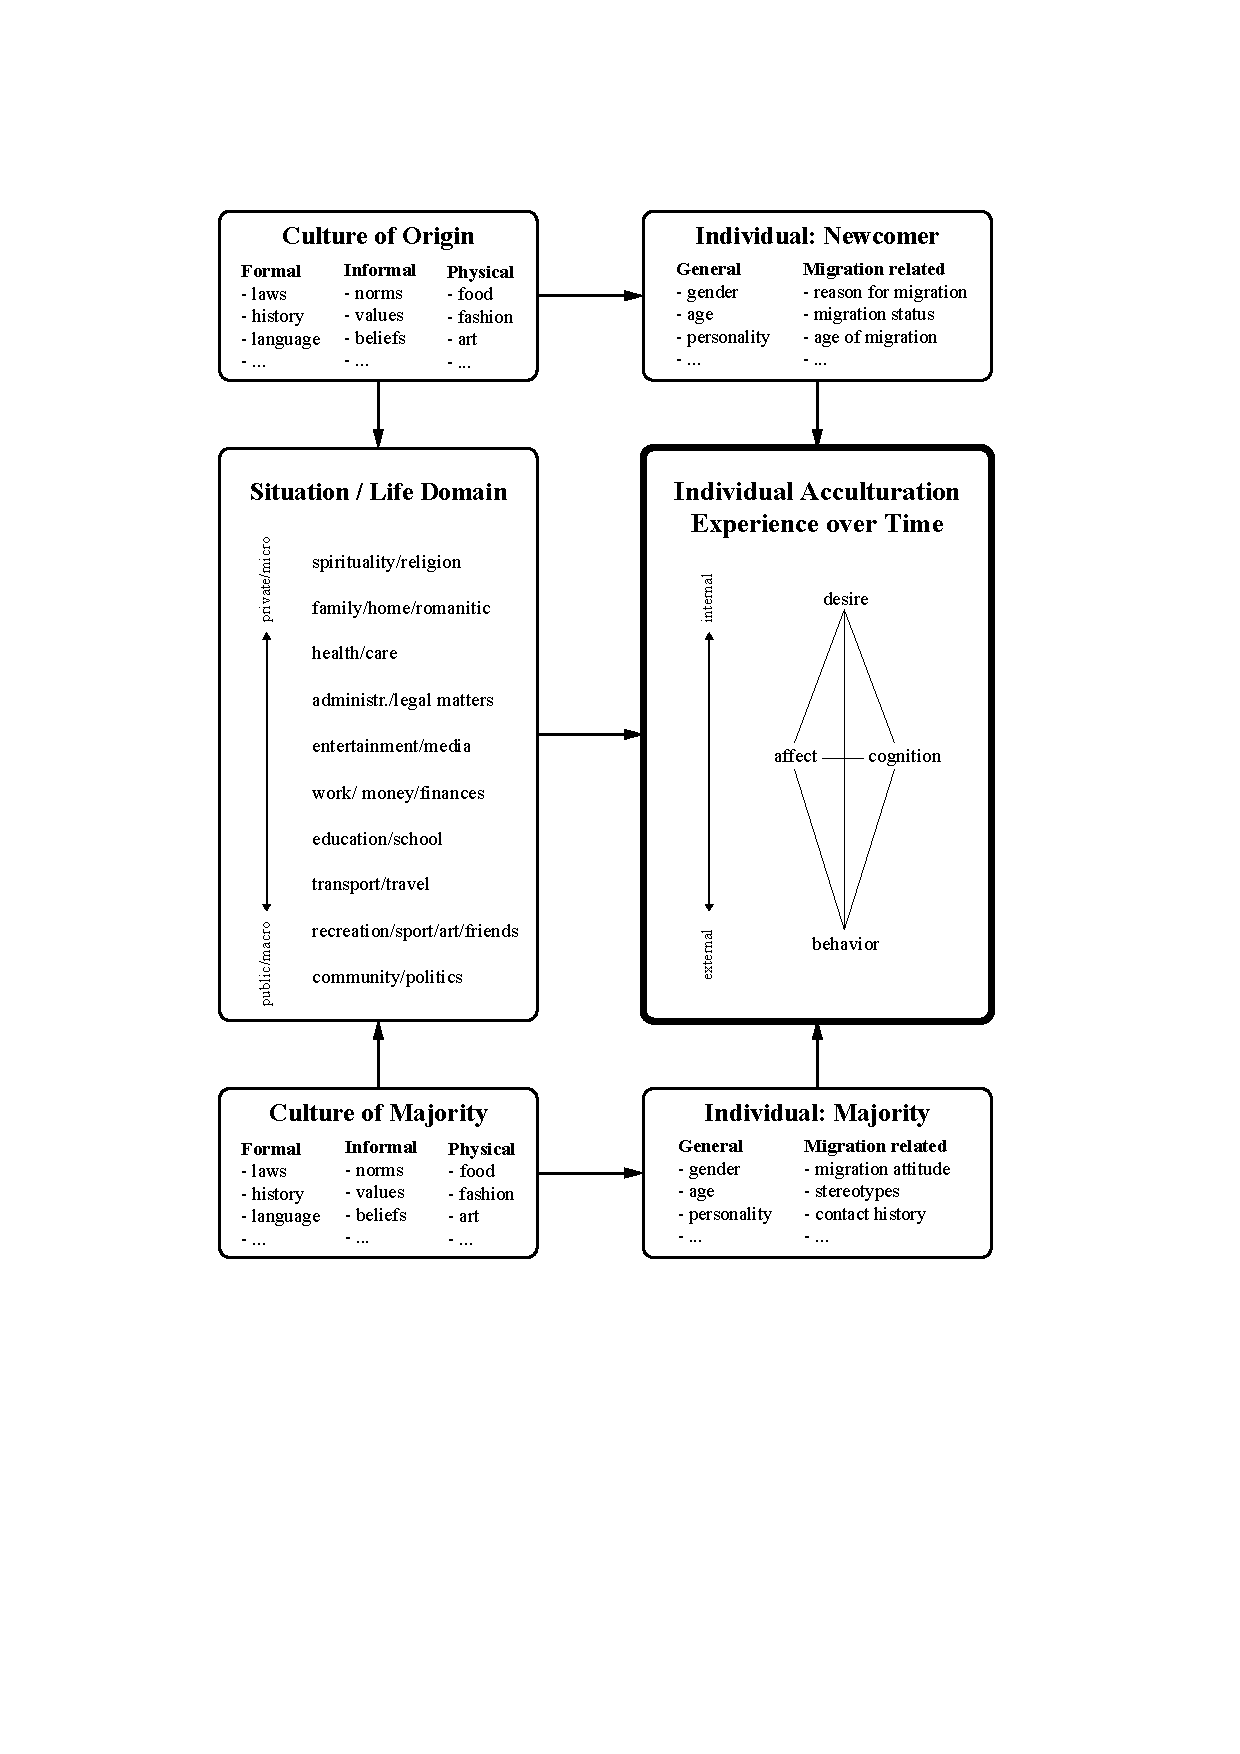
\includegraphics[width=\textwidth]{Figures/ConceptualFrameworkStatic.pdf}
\label{fig:ModelContext}
\end{figure}

\section{The Present Study}

%\begin{center}
%    \Warning\ \textsc{next sections not re-worked yet} \Warning
%\end{center}

The aim of our empirical efforts presented here is to put our proposed framework to the test. We have lamented that one of the challenges of a heterogeneous field is that it is difficult to assess and compare past literature. As a framework, we have suggested that the psychological elements of experiences could comprehensively structure our assessment of the literature. We will thus retrieve the past psychological literature on psychological acculturation and will extract which experiential aspects were considered in the research. We expect that these efforts will provide insights into the perceived importance of desires, affects, cognitions, and behaviors for psychological acculturation. We also expect that this allows us to assess how many experience aspects are usually considered and which aspects are considered jointly. And finally, we aim to compare the understanding of psychological acculturation across different fields to assess the comparative utility. 

To apply the framework, we specifically target three bodies of literature that capture the concept of psychological acculturation. Firstly, we will assess the theoretical literature on psychological acculturation. The theoretical literature should offer the broadest, most abstract, and most comprehensive works on psychological acculturation. A coding of the aspects considered in these theories should, thus, offer insights into the assumptions on which researchers build their empirical work.
Secondly, we will assess methodological literature developing acculturation measures. As operationalizations of the concept within the empirical literature, validated scales usually focus on a concept in a generalized manner, rather than focusing on aspects only relevant to a specific `applied' investigation. Coding psychological acculturation measures separately might also aid future considerations of measure selection because we effectively build a database of scales that can be filtered by whether the scale includes measurements of affects, behaviors, cognitions, and desires (see Supplemental Material D). 
Thirdly and finally, once we have considered the validated scales in particular, we will more generally assess the empirical literature that used measures of psychological acculturation. Capturing operationalizations within empirical studies, allows us to investigate the focus within the empirical literature more broadly and allows us to compare differences between fields and research subjects.

In the following section, we will briefly discuss how we conducted the systematic literature review and will sequentially analyze the role of experience elements in the theoretical, methodological, and empirical literature of psychological psychological acculturation\footnote{It should also be noted that we consciously chose not to conduct a meta-analysis. We conduct this review exactly because we are worried about comparability across studies, a key requirement of meta-analyses \citep{Pogue1998}. In our case, we, arguably, do not have a clearly defined concept and exclusions to ensure a cohesive data set would be counterproductive to our efforts. Moreover, a meta-analysis is commonly understood as an analysis of analyses \citep{Glass1976}. However, since we are interested in a conceptualization (rather than a relationship, a scale metric, or population parameter) a quantitative summary in form of a meta-analysis is not well-suited to answer our research question. Also a meta-analysis of our own extracted data seems profitless because it would likely mirror a sample size weighted average.}.

\section{Systematic Review}
% import methods and results from R Markdown (in file: "Methods-and-Results.tex")
\subsection{Methodological Literature}

Based on the systematic review and its coding, the first data set we
assess is a database of scale validations. We bring together the scales
suggested in previous reviews as well as validation studies we
identified in our own review. Throughout our literature review we found
five major works that reviewed the measurement of acculturation
\citep{Celenk2011, Maestas2000, Matsudaira2006, Wallace2010, Zane2004}.
After removal of duplicate scales, we added any scale validation that
was present in our own systematic review but not included in the
previous reviews. For each measure we extracted the full item list as
well as the item scoring prior to coding. A comprehensive and
interactive database of the scales, with reference- and publication
information, as well as our experience elements and -context coding is
available in our online supplementary information as well as on our open
science repository (\hl{OSF and/or github citation here}).

\subsubsection{Methods}

Taken together these five reviews collected a total of 197 scales, of
which 75 were duplicates. From our own review we added 25 additional
validation studies. After removing duplicates this meant that we
considered a total of 122 unique scales for our coding. Of these scales
we ultimately had to exclude 41, because they were either not accessible
or did not fit the the topic of our review (see Table
\ref{tab:ScalesExclusion}). The scales had an average of \hl{X.XX} items
and \hl{X.XX} sub-scales. Most items were rated on a five-point
(\hl{XX.XX}\%) or four-point likert-type scale (\hl{XX.XX}\%), with only
\hl{X} scales including categorical ratings. About a fifth of scales
(20.49\%) included majority group members in their validation studies.
The earliest included validation was from 1972 with a majority of scales
being validated around the turn of the 21\textsuperscript{st} century
and the latest included validation study in 2018.

\begin{table}

\caption{(\#tab:ScalesExclusion)Reasons for Exclusion}
\begin{tabular}[t]{lc}
\toprule
Exclusion Reason & Frequency\\
\midrule
not migration & 14\\
items not included & 8\\
search pending & 5\\
not accessible & 4\\
not found & 3\\
not acculturation & 2\\
majority focussed & 1\\
not found probably the same as Tsai et al. 2000 & 1\\
only language (no scale) & 1\\
same as S-029 & 1\\
uses other scale & 1\\
\bottomrule
\end{tabular}
\end{table}


\subsubsection{Results}

For the scale validations, we assessed both the role of experience
elements in the measures as well as contextual differences.

\paragraph{Experience}

With our main aim of examining the experience structure within the
scales, we examined whether scales included a specific experience
elements but also examined the used elements in their complex
combinations. In terms of general inclusion of elements, most studies
included a measure of cognition (89.66\%) and behavior (82.76\%),
whereas only roughly half the studies included a measure of affect
(55.17\%) and only a fourth of the scales included a measure of motives
(28.74\%). However, only a minority of scales included only a single
dimension. There were only 5 scales that exclusively relied on
cognitions (5.75\%) and 4 scales that measured only behaviors (4.6\%).
Yet, inversely, there were also only 13 scales that measured all four
dimensions (14.94\%). Most studies measured two (37.93\%) or three
(36.78\%) dimensions. A majority of scales either measured behavioral
and cognitive elements (26.44\%) or behavioral, cognitive, and affective
elements (26.44\%; also see Figure \ref{fig:ElementsScales} and Table
\ref{tab:ScaleElementCooccurrences}). Looking at the number of elements
measured together we also see substantial differences in what kind of
scales include a certain element. Scales that included cognitions
measured an average of 2.67 elements, scales measuring behavior, on
average, measured a 2.71, while scales that included affect measures had
a complexity average of 3.1 and scales measuring motivation even
measured an average of 3.4 scales. Thus, most scales measure multiple
dimensions, yet they focus on easily accessible dimensions (i.e.,
behavior and cognition), less of what is considered `less accessible' or
`subjective' (i.e., affect and desires). This is also visible in the
circumstance that there were no scales that exclusively measured
motivational or emotional adaptation (while this was the case for both
cognitions and behaviors). And if emotional or motivational aspects were
measured they were on average measured in scales that were already more
complex (i.e., included more experience elements).

\begin{figure}[h]
\centering
\caption{Scales: Bar graph of the experience element combinations.}
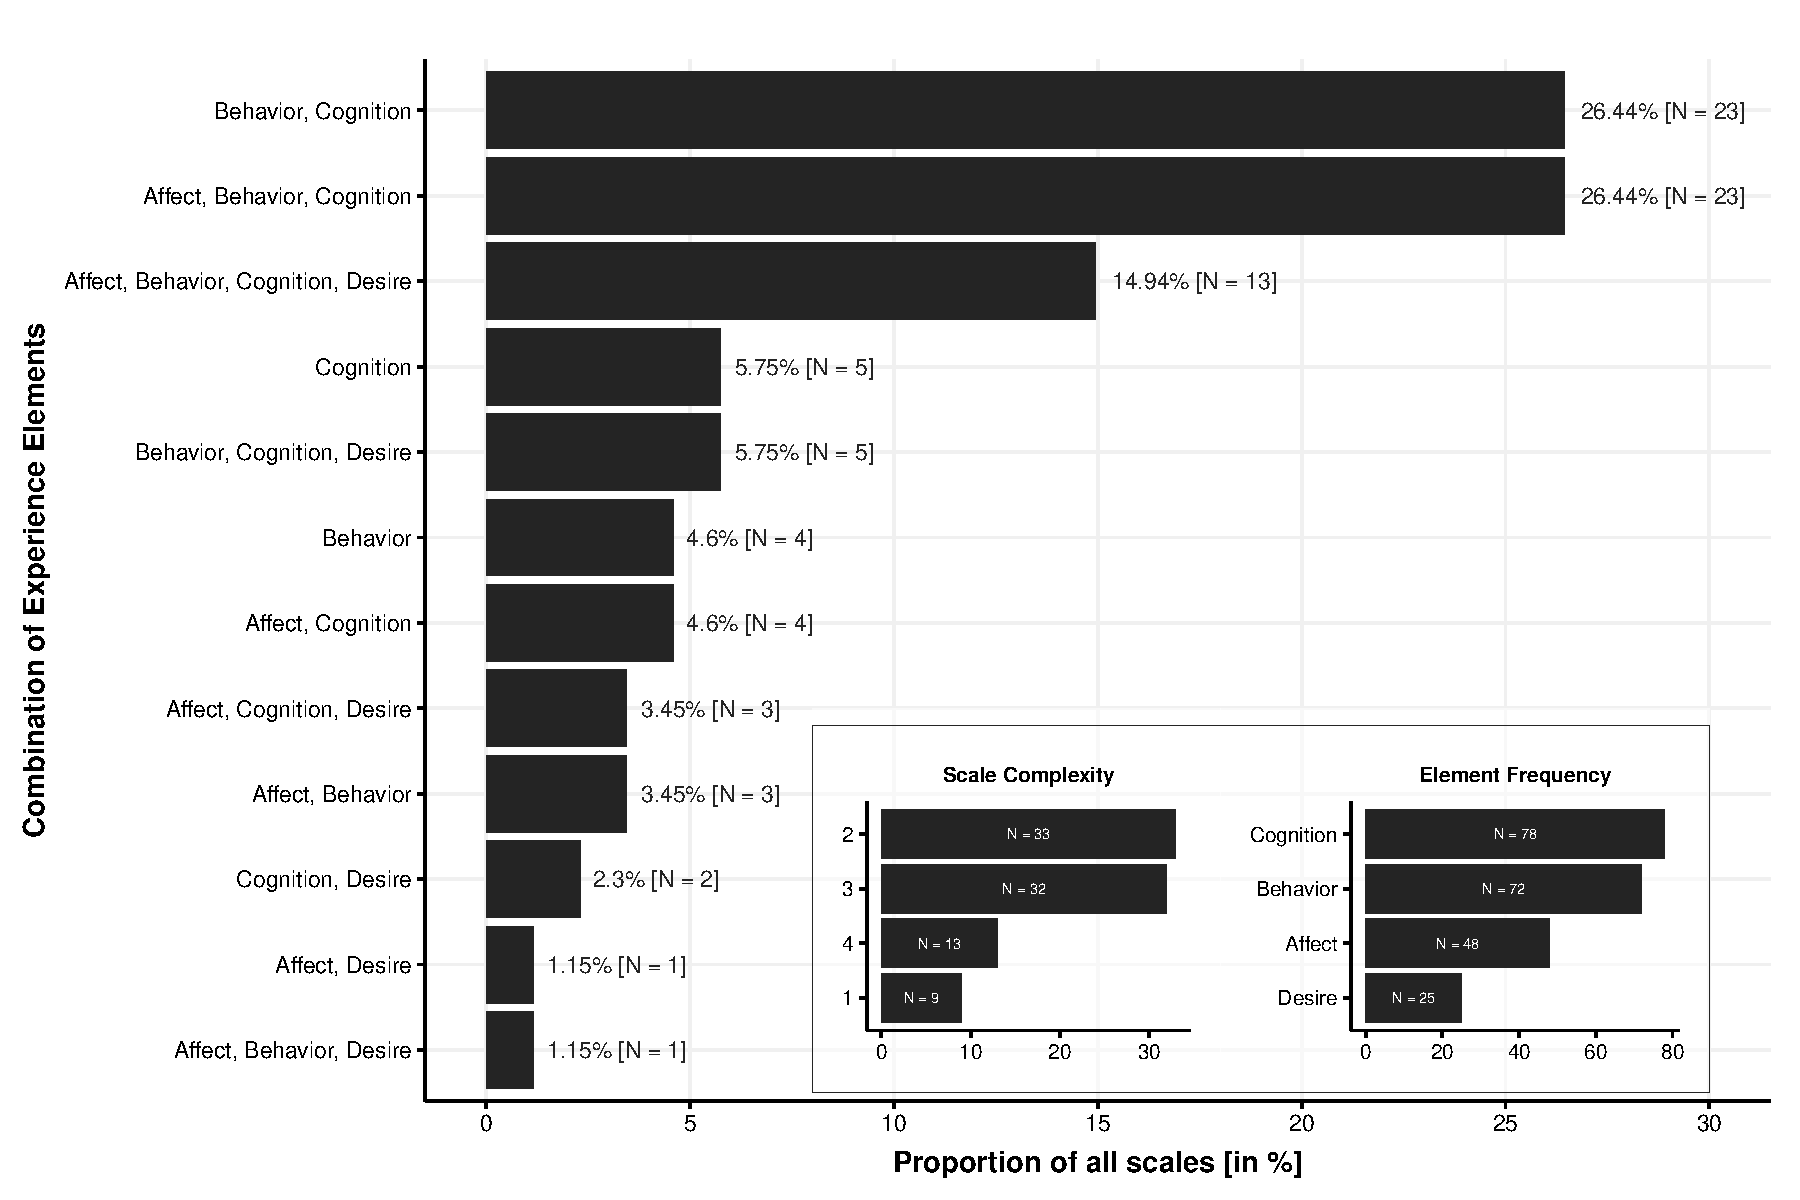
\includegraphics[width=\textwidth]{Figures/ABCDFreq-1}
\label{fig:ElementsScales}
\end{figure}

\begin{table}

\caption{\label{tab:ScaleElementCooccurrences}Scales: Element Co-occurrence Matrix}
\begin{tabular}[t]{lcccc}
\toprule
  & Affect & Behavior & Cognition & Desire\\
\midrule
Affect & 48 & 40 & 43 & 18\\
Behavior & 40 & 72 & 64 & 19\\
Cognition & 43 & 64 & 78 & 23\\
Desire & 18 & 19 & 23 & 25\\
\bottomrule
\end{tabular}
\end{table}

\paragraph{Context}

To gain a general understanding of contextual factors within the
validated studies, we also assessed cross-study patterns of cultural,
individual, situational, and process-related focus points.

\subparagraph{Country}

To assess the cultural contexts for which scales were validated, we
assessed the migrants' countries of settlement as well as the countries
of origin. We found that most scales investigated a single host country
(\textit{N} = 81) and most investigated one country of origin
(\textit{N} = 68). There were only 3 scales that were validated for more
than one receiving country. Additionally, there was one study with two
scales that were validated with the origin culture as the starting point
(i.e., single origin country, multiple host countries). Looking at the
country patterns, we found that an overwhelming number of scales were
validated within a U.S. American settlement context (\textit{N} = 61).
But also the remaining receiving societies were mostly `western'
countries (e.g., Canada, The Netherlands, The United Kingdom, Israel,
Australia) with non-western settlement contexts, such as Taiwan, Nepal,
or Russia, not being investigated across more than one study. For the
migrant origin societies there was slightly more variation. There were a
few migrant groups that were investigated specifically (e.g., Mexico:
14, China:7, South Korea: 4), however most validation studies targeted
broader categories of migrants (any migrants: 11, Asian: 5, Hispanic: 9,
LatinX: 5). This also made it difficult to identify patterns of cultural
combinations investigated (apart from Mexican and LatinX migrants in the
United States).

\subparagraph{Sample}

To assess the role different groups of individuals targeted in the scale
validations, we coded the types of samples recruited for the validation
studies. A majority of studies sampled any consenting adult from the
migrant group of interest (\textit{N} = 50). As seems common in academic
research, a larger portion of the validated scales relied on young
migrants or students (\textit{N} = 29). Interestingly, only small
minority of validated scales targeted more vulnerable groups, such as
clinical samples (\textit{N} = 2) or refugees (\textit{N} = 2) --
despite a considerable focus on these groups within the broader
literature.

\subparagraph{Domains}

To assess the situational focus within the validated scales, we assessed
the number of domains within each scale as well as more common domains
across the scales. A relatively large number of scales asked about the
current state of the migrant in general manner without mentioning any
context or life domain (\textit{N} = 24; e.g., `'In general, in what
language do you read and speak?'`). The remaining scales referred to an
average of 3.49 dimensions (\textit{SD} = 3.42, range: 1 -- 21). A total
of 179 unique domains was measured across the 87 scales. The domains of
'language` (\hl{XX}\%), 'food' (\hl{XX}\%), `interactions' (\hl{XX}\%),
`family' (\hl{XX}\%) and `values' (\hl{XX}\%) were focused on most often
(see Online Supplementary Materials \hl{X}, Figure \hl{X}). Thus, while
there was large variation between the scales in the number, and
diversity of domains, the most frequently mentioned domains were in line
with the life domains proposed in the literature
\citep[e.g.,][]{Arends-Toth2007}.

\vspace{1em}
\todo[inline]{Should be re-coded to test our proposed domains. Also, re-check `general' code}

\subparagraph{Migration time}

All scales were validated using cross-sectional data after the migrant
arrived in the settlement society. This is in line with observations by
previous reviews of the field \citep[e.g.,][]{Brown2011}.

\subsection{Empirical Literature}

After analysis of the scales validations, we assessed the broader
empirical works we collected within the systematic review. We first
looked at all available empirical publications (incl.~books, chapters,
and dissertations). We later also assessed differences between fields
the work was published in. However, because we considered the fields on
an audience level, we used only empirical journal articles -- for which
journal-level audience data is available.

\subsubsection{Methods}

The search produced a total of \hl{XXX} results to which we added
\hl{XX} articles through contacts with experts in the field. We
subsequently screened out results that did not fit into our review.
After duplicate removal (\(N_{excluded}\) = \hl{XX}, \(N_{screened}\) =
484), we excluded 92 results in the title screening as well as an
additional 126 results during the abstract screening. Of the remaining
266 results, 259 papers presented empirical work on acculturation and
were coded. The 7 non-empirical results were reviews, which were not
coded because they did not fit into our coding schema. During the full
text coding we excluded an additional 26 results because they were
either not relevant or were not accessible (for exclusion reasons see
Table \ref{tab:EmpiricalExclusion} and for our PRISMA diagram see Figure
\ref{fig:PRISMA}).

\begin{figure}[h]
\centering
\caption{PRISMA diagram. Position still undecided. Currently generated in R based on n(row) maybe make prettier. \Warning\ Re-check numbers before duplicates removed and number of papers added from other sources.}
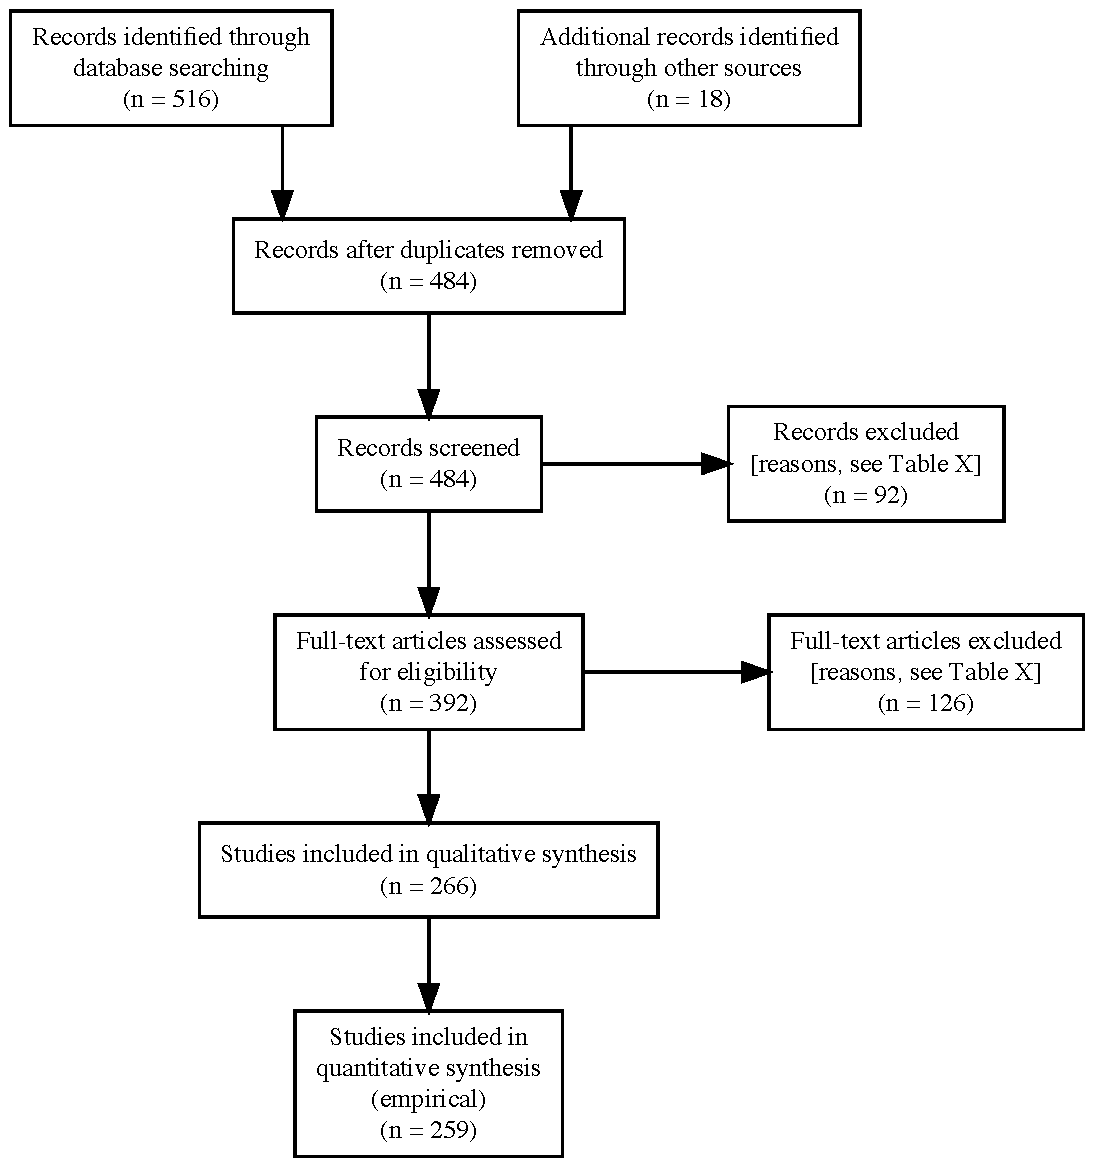
\includegraphics[width=\textwidth]{Figures/PRISMA}
\label{fig:PRISMA}
\end{figure}

\begin{table}

\caption{\label{tab:EmpiricalExclusion}Exclusion Reasons Empirical Literature}
\centering
\begin{tabular}[t]{lccc}
\toprule
\multicolumn{1}{c}{ } & \multicolumn{3}{c}{Screening} \\
\cmidrule(l{3pt}r{3pt}){2-4}
Exclusion Reason & Title & Abstract & Full Text\\
\midrule
not migration & 36 & 27 & \\
not acculturation & 19 & 49 & \\
not experience & 19 & 24 & \\
not migrant & 17 & 18 & \\
not measured &  & 8 & 2\\
re-migration &  & 1 & \\
thesis not accessible &  &  & 13\\
book not accessible &  &  & 4\\
items not accessible &  &  & 4\\
article not accessible &  &  & 2\\
should still be coded &  &  & 1\\
\bottomrule
\end{tabular}
\end{table}


Of the final works we coded, 192 were journal articles, 37 theses, and 4
book chapters. Most studies presented quantitative data (\textit{N} =
205), mixed methods (\textit{N} = 14), or qualitative data (\textit{N} =
11), while the remaining 3 manuscripts were reviews of empirical data. A
vast majority of the authors used the term `acculturation' (or
derivative versions, such as `acculturation attitudes' or `acculturation
orientation'; \textit{total N} = 178), or `integration' (\textit{N} = 7)
to refer to cultural adaptation. Notably, a majority of the empirical
investigations did not share common measures of cultural adaptation --
186 studies used measures that were reported a maximum of five times,
with a considerable majority of papers using new or ad-hoc measures of
cultural adaptation. Only about every tenth study included the local
majority in the study (\textit{N} = 25, 10.8225\%). Cultural adaptation
most frequently was a predictor variable (\textit{N} = 99, 42.8571\%), a
dependent variable (\textit{N} = 72, 31.1688\%), or a correlation
variable (\textit{N} = 27, 11.6883\%) in the empirical works. This
pattern was mirrored when looking at the focus of the papers, where a
majority of the papers had acculturation as their main focus (\textit{N}
= 83, 36.7257\%), with other bodies of work focusing on health outcomes
(\textit{N} = 23, 10.177\%), or inter-group relations (\textit{N} = 12,
\texttt{empFocusRelationPerc}\%) as their main outcomes. The earliest
included study was published in 1970, with a continuous increase of
publications after the year 2000, with considerable publication peaks in
2011 and 2019. We provide full descriptions of descriptive data
extractions and additional information about the data description in
Online Supplementary Information X.

\paragraph{Field of Publication}

For the broader empirical literature, we also collected additional data
on the field the studies were published in. To assess the differences
between fields we merged the `Scimago Journal Ranking Database'
\citep{SCImago2020} with our empirical review. For all available journal
articles we added information on key journal metrics (incl.~H index,
impact factor, and data on the field and audiences). This also meant
that dissertations, book chapters, and books were excluded from this
analysis because data on their publishers is not readily available or
unreliable. Additionally, 8 journals were not included in the Scimago
database (likely because they do not have an ISSN identifier or were
discontinued before 1996, see Online Appendix \hl{X}, Table \hl{X} for
the missing journals). We ultimately had journal metrics for 183
empirical articles. The Scimago database classifies each journal
according to the field(s) that the journal aims to address. Importantly,
(1) each journal can be be classified to address multiple fields and (2)
the field include codes of fields (e.g., `Social Sciences') as well as
sub-fields (e.g., `Social Psychology'). This leads to the case that
there can be substantial overlap between fields, and journals cannot
easily or readily be assessed in mutually exclusive subgroups.

To summarize the articles further we then classified the field
combinations into super-ordinate discipline codes. These discipline
codes are based in part on U.S. Department of Education's subject
classifications \citep[i.e., CIP;][]{InstituteofEducationSciences2020},
the U.K. academic coding system
\citep[JACS 3.0;][]{HigherEducationStatisticsAgency2013}, the Australian
and New Zealand Standard Research Classification
\citep[ANZSRC 2020;][]{AustralianBureauofStatistics2020}, as well as the
Fields of Knowledge project \citep{ThingsmadeThinkable2014}. We
ultimately classified each journal into one of four mutually exclusive
disciplines (psychology: \textit{N} = 61, multidisciplinary: \textit{N}
= 57, Medicine, Nursing, and Health: \textit{N} = 51, and Social
Sciences (miscellaneous): \textit{N} = 14. For a full discussion of the
classifications see Online Supplementary Materials \hl{X}).

\subsubsection{Results}

To test the utility of our framework, we again assessed the role of
experience elements in the measurement as well as contextual
differences.

\paragraph{Experience}

In terms of the overall frequencies of experience elements, the broader
empirical data mirrored that of the validation studies. Most studies
included a measure of cognition (83.26\%) and behavior (80.69\%),
whereas only about half of all studies included a measure of affect
(51.93\%) and only a fifth of the studies included a measure of motives
(18.45\%). Yet, only 42 studies focused on a single element
(\(N_{behavior\ only}\) = 20, \(N_{cognition\ only}\) = 18,
\(N_{emotion\ only}\) = 4). Similarly, only 17 papers included measures
of all four experience elements (7.3\%). Most studies measured three
(37.77\%) or two dimensions (36.91\%). Different from the scale
validations, within the broader empirical works most works included
measures of emotions, behaviors, and cognitions (\textit{N} = 69,
29.61\%), with a further substantial number of articles measuring
behaviors and cognitions (\textit{N} = 53, 22.75\%. Also see Figure
\ref{fig:EmpPlotFreq-1} and Table
\ref{tab:EmpiricalElementCooccurrences}). Looking at the number of
elements measured together we again see substantial differences in what
kind of scales include the individual elements. Scales that included
cognitions measured an average of 2.53 elements, scales measuring
behavior, on average, measured a 2.52, while scales that included affect
measures had a complexity average of 2.86 and scales measuring
motivation even measured an average of 3.23 scales. Thus, interestingly,
not a single study measured only motivation, and measures of motives
remained mostly limited to scales that were already multidimensional.
The results exacerbate the pattern found in the scale validations,
complex measures and conceptions of acculturation are seen infrequently
and readily accessible (i.e., less subjective) dimensions of cognition
and behavior remain the focus of most studies.

\begin{figure}[h]
\centering
\caption{Empirical Literature: Bar graph of the experience element combinations.}
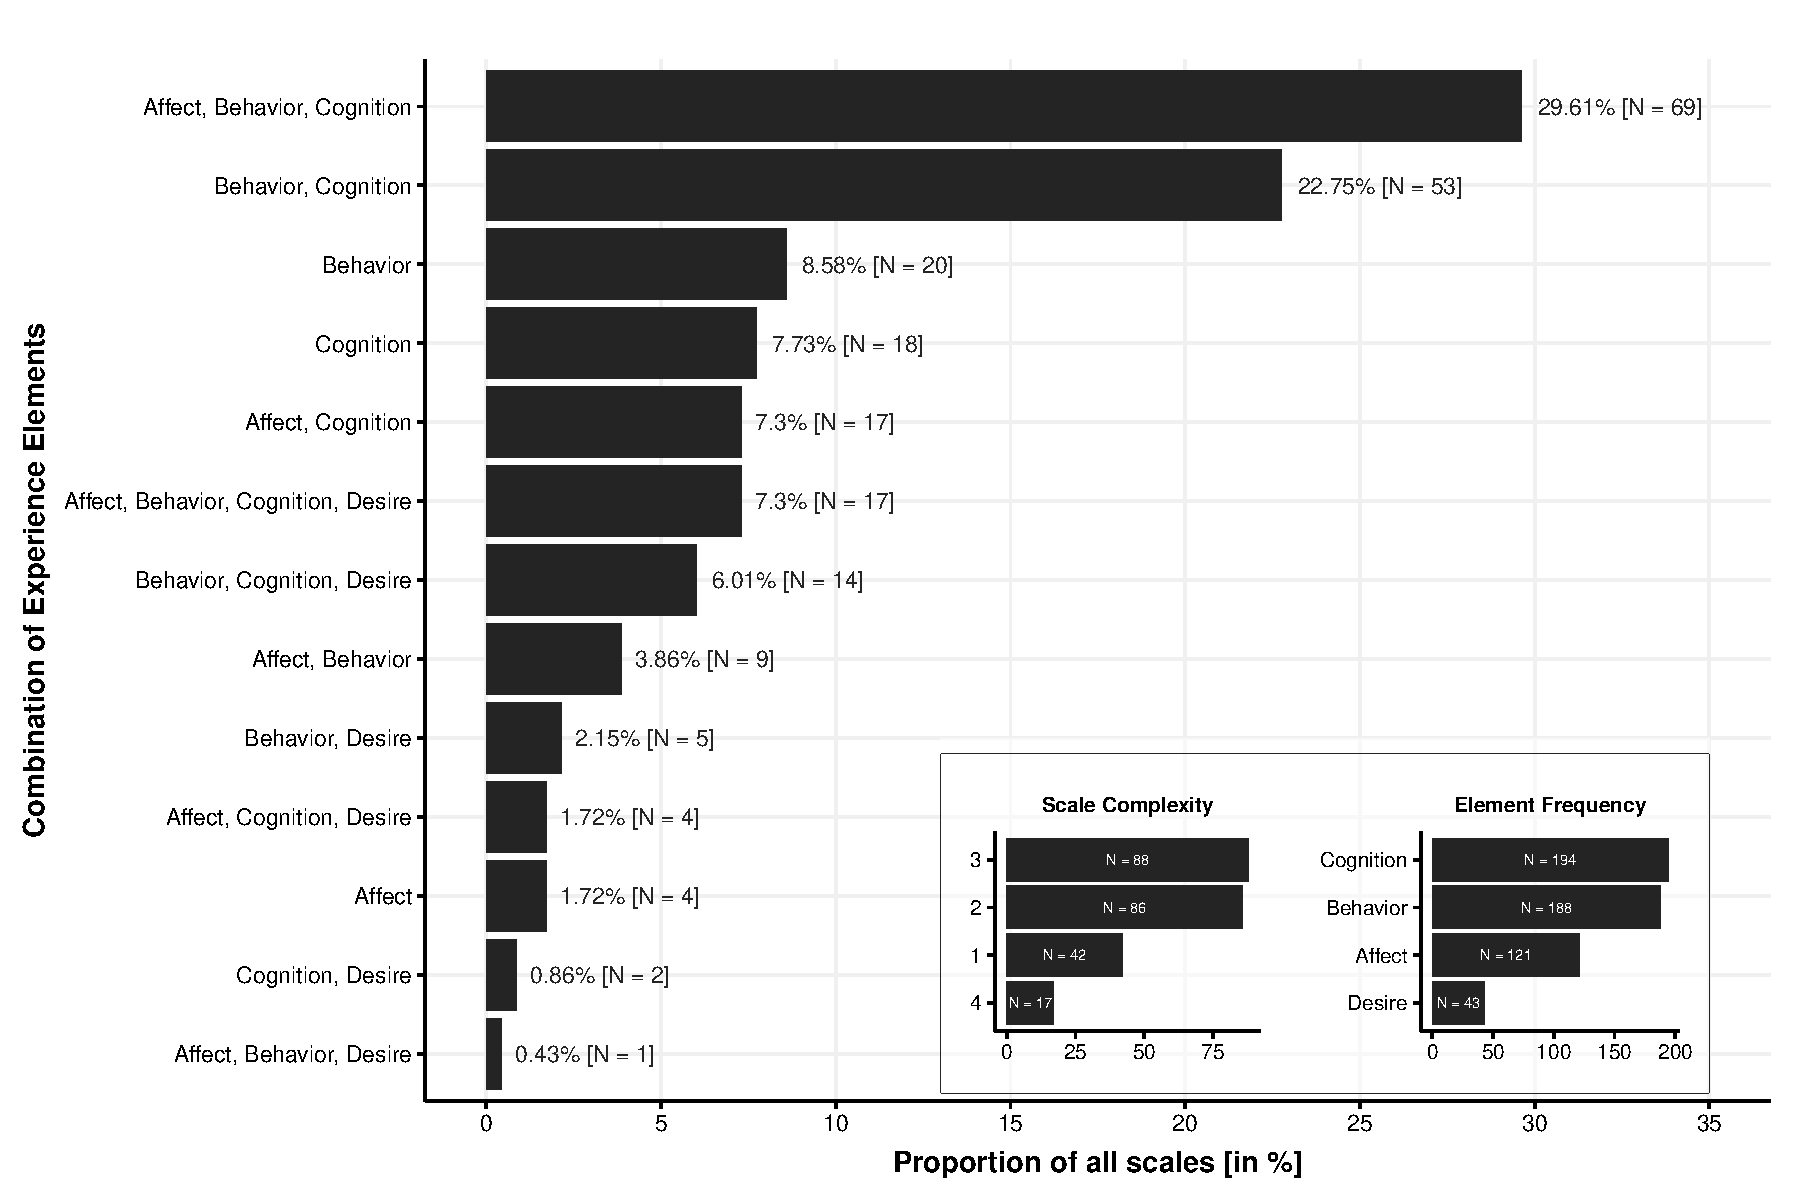
\includegraphics[width=\textwidth]{Figures/EmpPlotFreq-1}
\label{fig:EmpPlotFreq-1}
\end{figure}

\begin{table}

\caption{\label{tab:EmpiricalElementCooccurrences}Empirical Literature: Element Co-occurrence Matrix}
\centering
\begin{tabular}[t]{lcccc}
\toprule
  & Affect & Behavior & Cognition & Desire\\
\midrule
Affect & 121 & 96 & 107 & 22\\
Behavior & 96 & 188 & 153 & 37\\
Cognition & 107 & 153 & 194 & 37\\
Desire & 22 & 37 & 37 & 43\\
\bottomrule
\end{tabular}
\end{table}


\paragraph{Context}

To gain a general understanding of contextual factors within the broader
empirical studies, we again assessed cross-study patterns of cultural,
individual, situational, and process-related focus points.

\subparagraph{Country}

To assess the cultural contexts on which the authors focused, we again
assessed the migrants' countries of settlement as well as the countries
of origin. Similar to the validations, an overwhelming number of scales
were validated within a North American settlement context (United
States: \textit{N} = 109, Canada: \textit{N} = 26). But also the
remaining receiving societies were mostly `western' -- Western Europe
(e.g., The Netherlands, United Kingdom, Germany, Italy, Spain),
Australasia (Australia, New Zealand), Russia, and Israel. And only 10
studies focused on data from multiple receiving societies.

When it came to the migrants' country of origin, a majority of studies
were indifferent to migrants background and simply recruited any
consenting migrant (\textit{N} = 37), or recruited a category of
migrants (e.g., LatinX or Hispanic: \textit{N} = 21, African: \textit{N}
= 10). Among the individual countries target there was a particular
focus on the east and south-east Asian region (e.g., China: \textit{N} =
21, South Korea: \textit{N} = 19, Vietnam: \textit{N} = 11). Yet,
different from the scale validations, there was a large variety of
different origin countries that were included in less than five studies
(\textit{N} = 101 regions were targeted less than five times). Thus, the
receiving countries mainly mirrored those for which scales were
validated, yet there was an extensive number origin countries which were
investigated individually or migrants were considered irrespective of
their cultural origin. Moreover, it was again not possible to identify
distinct cultural adaptation clusters within the literature (that would
be large enough to compare).

\subparagraph{Sample}

To assess the role different groups of individuals targeted in the
empirical work, we again coded the types of samples recruited for the
studies. A majority of studies sampled any consenting adult from the
migrant group of interest (\textit{N} = 145, 62.23\%). Of the targeted
sampling strategies, most recruited refugees (\textit{N} = 22, 9.44\%),
young migrants (\textit{N} = 20, 9.01\%), or elderly people (\textit{N}
= 14, 6.01\%). The remaining fifth of the studies recruited other more
specific samples (e.g., nurses, athletes, Muslims). Interestingly,
despite the circumstance that a large portion of papers focused on
mental health outcomes, only 7 studies (3\%) recruited clinical migrant
samples. These results speak to the case that relatively few empirical
studies actually take individual differences into account in their
sample selection. Studies may still address individual differences
within the data description and within the modeling approaches (e.g.,
controlling for gender), yet it seems that inter-sectional
idiosyncrasies did not seem to play a major role in the targeting of
samples.

\subparagraph{Domains}

To capture the situational focus of the authors, we coded which life
domains the utilized measures referred to. A relatively large number of
studies assess cultural adaption in general manner without mentioning
any context or life domain (\textit{N} = 116). The remaining studies
referred to an average of 2.16 dimensions (\textit{SD} = 2.69, range: 1
-- 21)). We found a total of 183 unique domains across the 233 studies.
The dimensions of `language` (\hl{XX}\%), 'food' (\hl{XX}\%), `social
interactions,' and `friends' (\hl{XX}\%) were included most frequently.
So, while larger proportion of studies ask about cultural adaption in
general (outside of a specific domain), the number of domains included
and addressed is extensive and diverse. The mentioned domains at times
go beyond the life fields mentioned in previous work (also see Online
Supplementary Materials \hl{X}).

\vspace{1em}
\todo[inline]{Should be re-coded to test our proposed domains. Also, re-check `general' code}

\subparagraph{Process}

To assess the process focus of the broader empirical works, we again
assessed when in the migration process was collected and we additionally
assessed the type analysis done by the authors. We found that a 224
studies (96.97\%) collected cross-sectional data after the arrival of
the migrant in the new society. A single study targeted potential
migrants and 6 studies collected data prior and following the migration
event. Moreover, only 3 studies included longitudinal data analyses
concerned with cultural adaptation. This observation, again underscores
the arguments made by authors, who have long pointed out that the
acculturation literature has thus far failed to provide data that
meaningfully captures migration as a process
\citep[e.g.,][]{Brown2011, Ward2019}.

\paragraph{Fields}

To further test the utility of our framework in comparing
conceptualizations, we assessed differences of experience elements
across different fields. We provide more elaborate descriptions of the
differences in the methods, and publication types as well as contextual
differences in terms of sampling procedures, situational domains,
process-focus, analyses, and cultural contexts in Supplementary Online
Material \hl{X}.

We again first, assessed the references to affect, behavior, cognition,
and desires separately, within each of the disciplines. We find that for
all fields motivations (14.29-22.95\% of all measures in the field) and
emotions (42.86-55.74\%) are the least frequently measured elements and
each of the fields measures similarly often (in proportional terms).
However, for the cognitive and behavioral elements the proportions
diverge between the fields. While the multidisciplinary field measured
behaviors (78.95\%) and cognition (80.7\%) almost equally often, in the
medical and general social science journals behaviors were measured
considerably more often than cognitions (\(Behavior_{SoSci}\) = 100\%
\textgreater{} \(Cognition_{SoSci}\) = 50\%; \(Behavior_{Med}\) = 90.2\%
\textgreater{} \(Cognition_{Med}\) = 76.47\%). While the psychological
journals cognitions (91.8\%) were measured more often than behaviors
(70.49\%; also see Figure \ref{fig:FieldPlotFreq} B and A)).

When looking at differences in how many different elements were measured
(i.e., element complexity) and patterns within these
element-combinations, differences between the fields become increasingly
evident (also see Figure \ref{fig:FieldPlotFreq} A and C). While
`affect, behavior, and cognition' and `behavior, and cognition' measures
are the most common combinations across all fields (also at similar
proportional importance), there is less dimension complexity and
variation for medical and social science fields. In the psychological
85.25\% of all studies measures at least two experience elements
(\textit{M} = 2.41, \textit{SD} = 0.68). Although mean complexity
differences were not significantly different between the fields
(\textit{F}(3, 179) = 0.63, \textit{p} = 0.599), looking at the
qualitative differences of element combinations can be informative. For
example, there was not a single study published in a psychological
journal that conceptualized cultural adaptation by behavior alone
(eventhough this is the third most common measures in the other three
fields, also see Figure \ref{fig:FieldPlotFreq} A). Similarly, in the
broader social scientific journal desires are always measured together
with behaviors, which is very uncommon in the other
fields\footnote{Although it should be noted that the social science field was smaller and more heterogeneous than the other fields. \Warning\ Maybe drop this argument -- based on only two studies.}.
There are also interesting pattern when one considers how many other
elements an aspect is measured with within each of the fields. For
example, while for all fields motivations are found in the most complex
scales
\footnote{except for the broader social science journals that do not have many motivational measures to begin with.},
medical journal have a substantially higher average scale complexity
when measuring motivations. Inversely, psychological journal on average
report behavioral measures of cultural adaptation in more complex
scales. This hints to a pattern, where complexity might indicate
relative importance of an aspect within the field -- where only scales
that already have a broad and diverse measure also include the elements
that are usually measured less within a field (also see Figure
\ref{fig:FieldElementComp}). There are like other and more nuanced
differences in the conceptualizations highlighted within this analysis
(e.g., patterns relevant to a single field). Yet, the immediately
visible pattern differences clearly speak the utility of the framework.

\begin{figure}[h]
\centering
\caption{Combinations of measured experience element and their frequencies per field.}
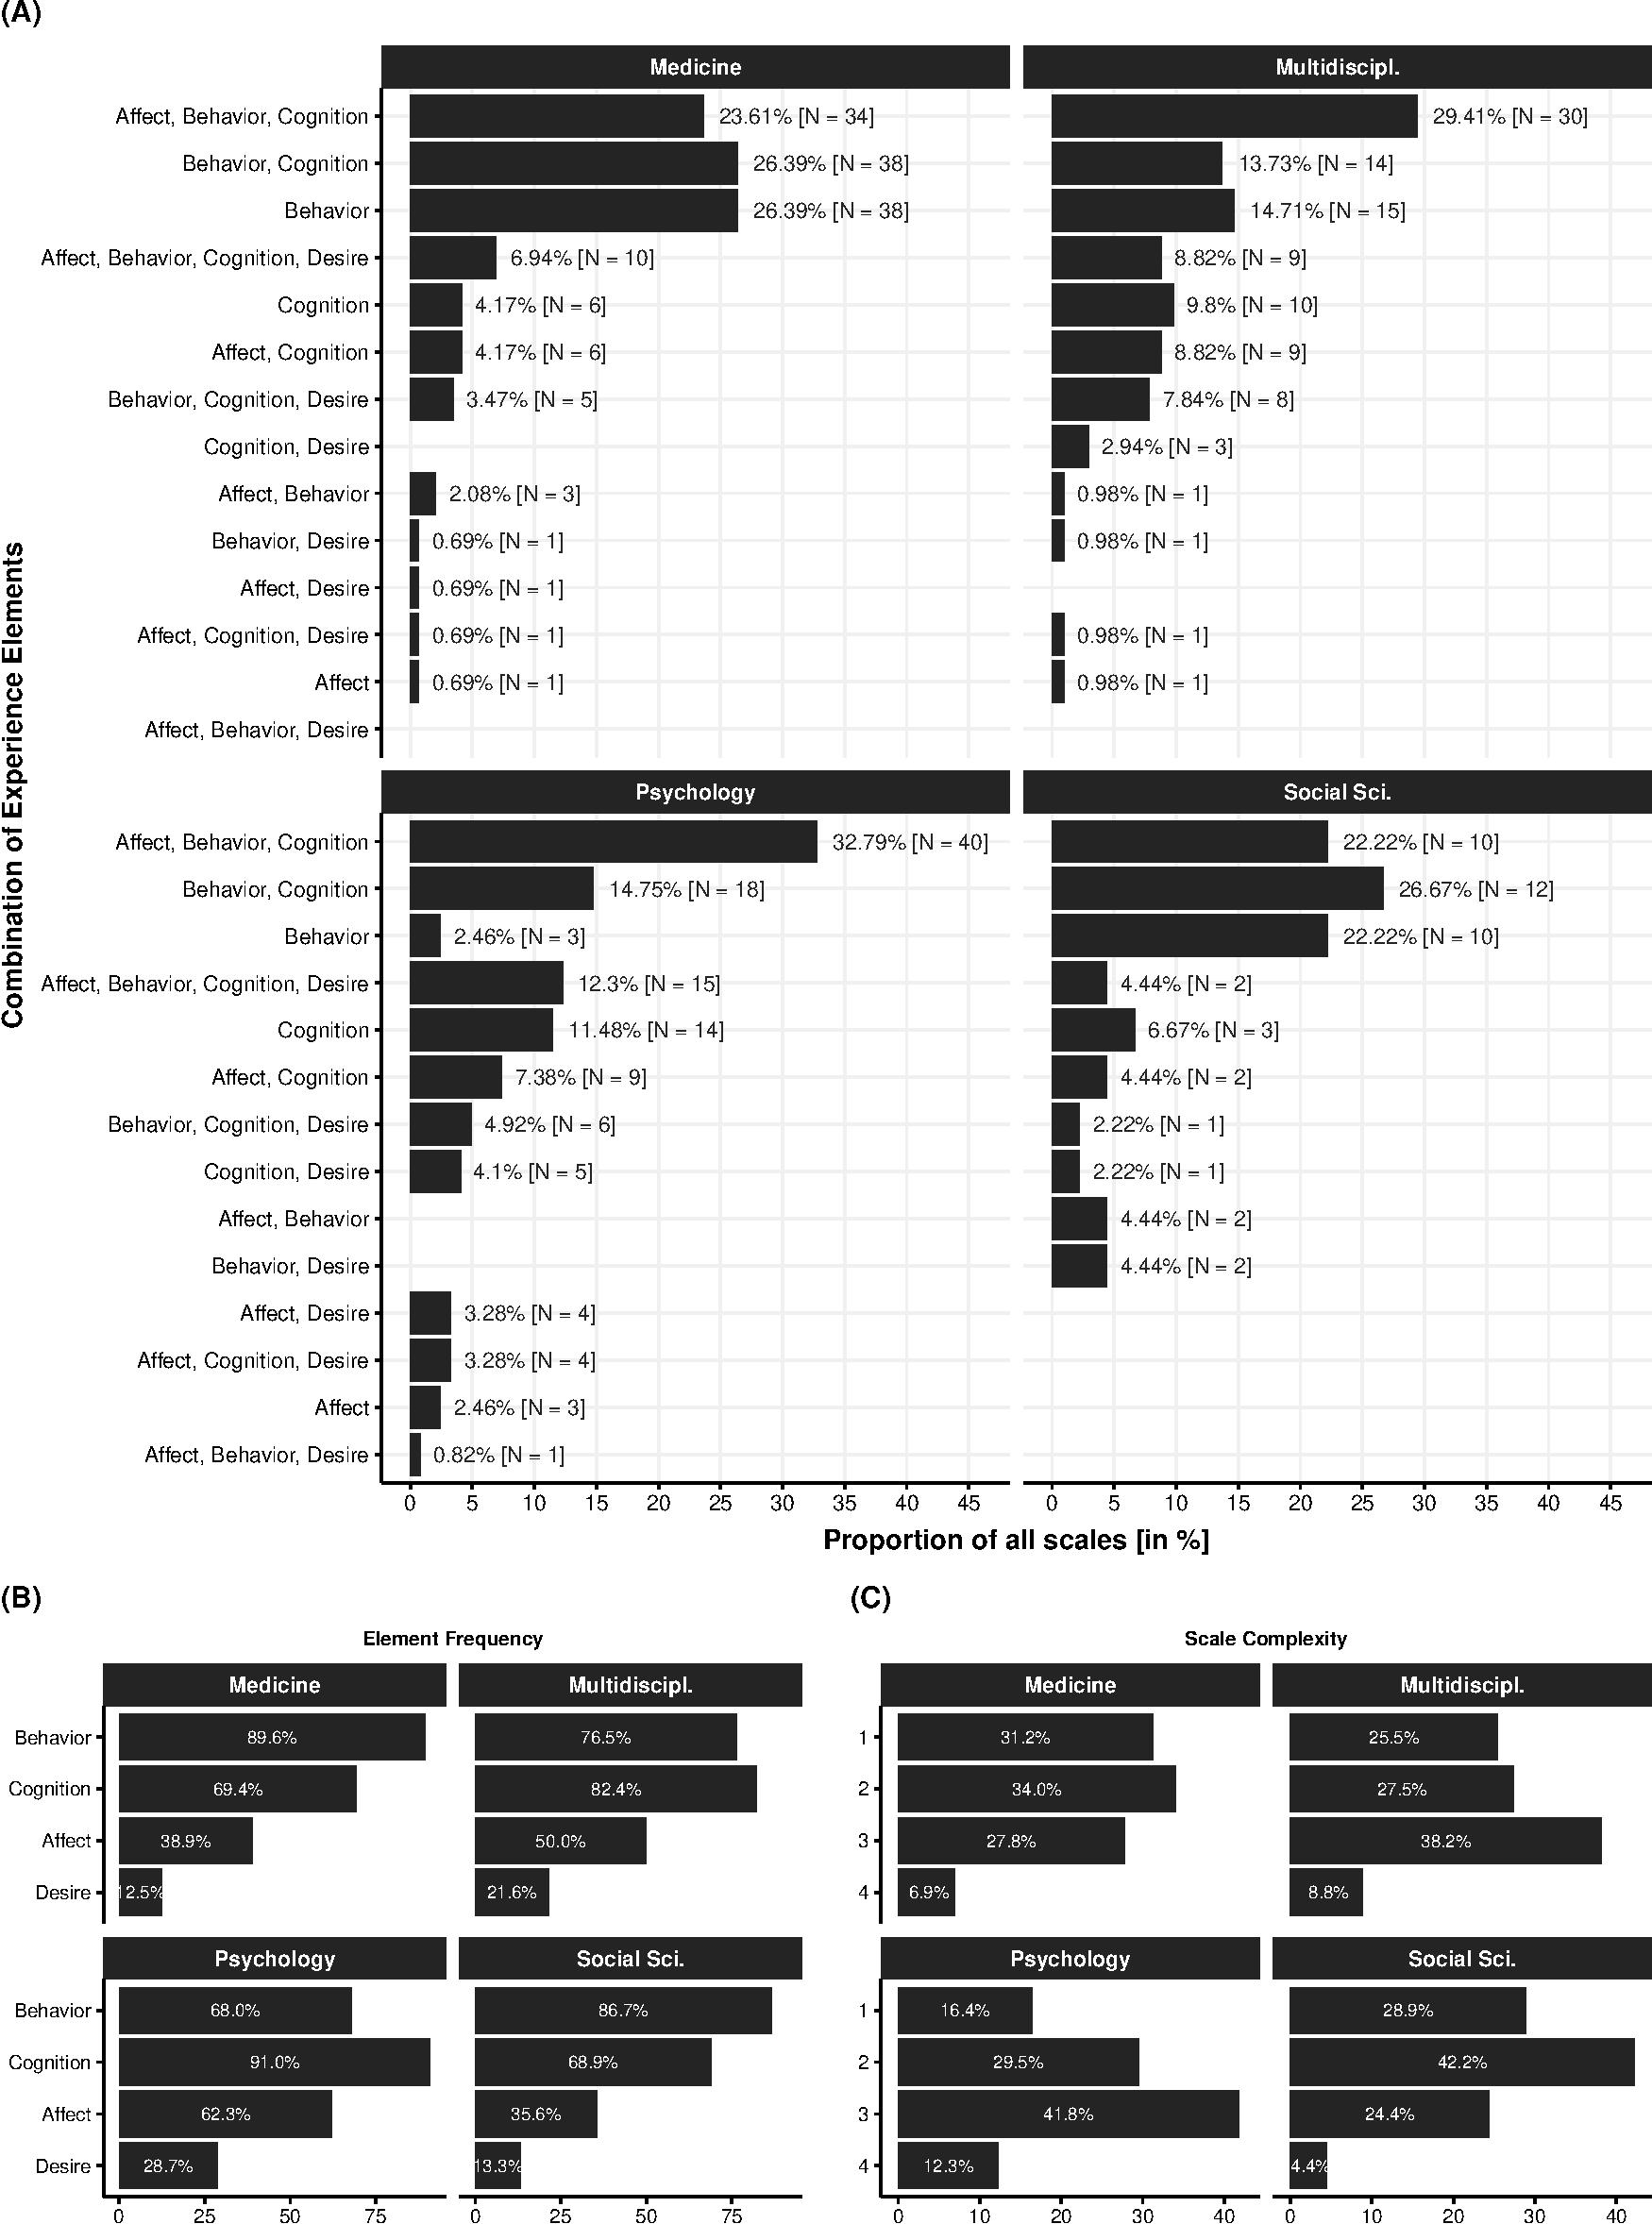
\includegraphics[width=\textwidth]{Figures/FieldPlotFreq-1}
\label{fig:FieldPlotFreq}
\end{figure}

\begin{figure}[h]
\centering
\caption{Average complexity (number of experience elements measured) for all scales that include a given experience aspect.}
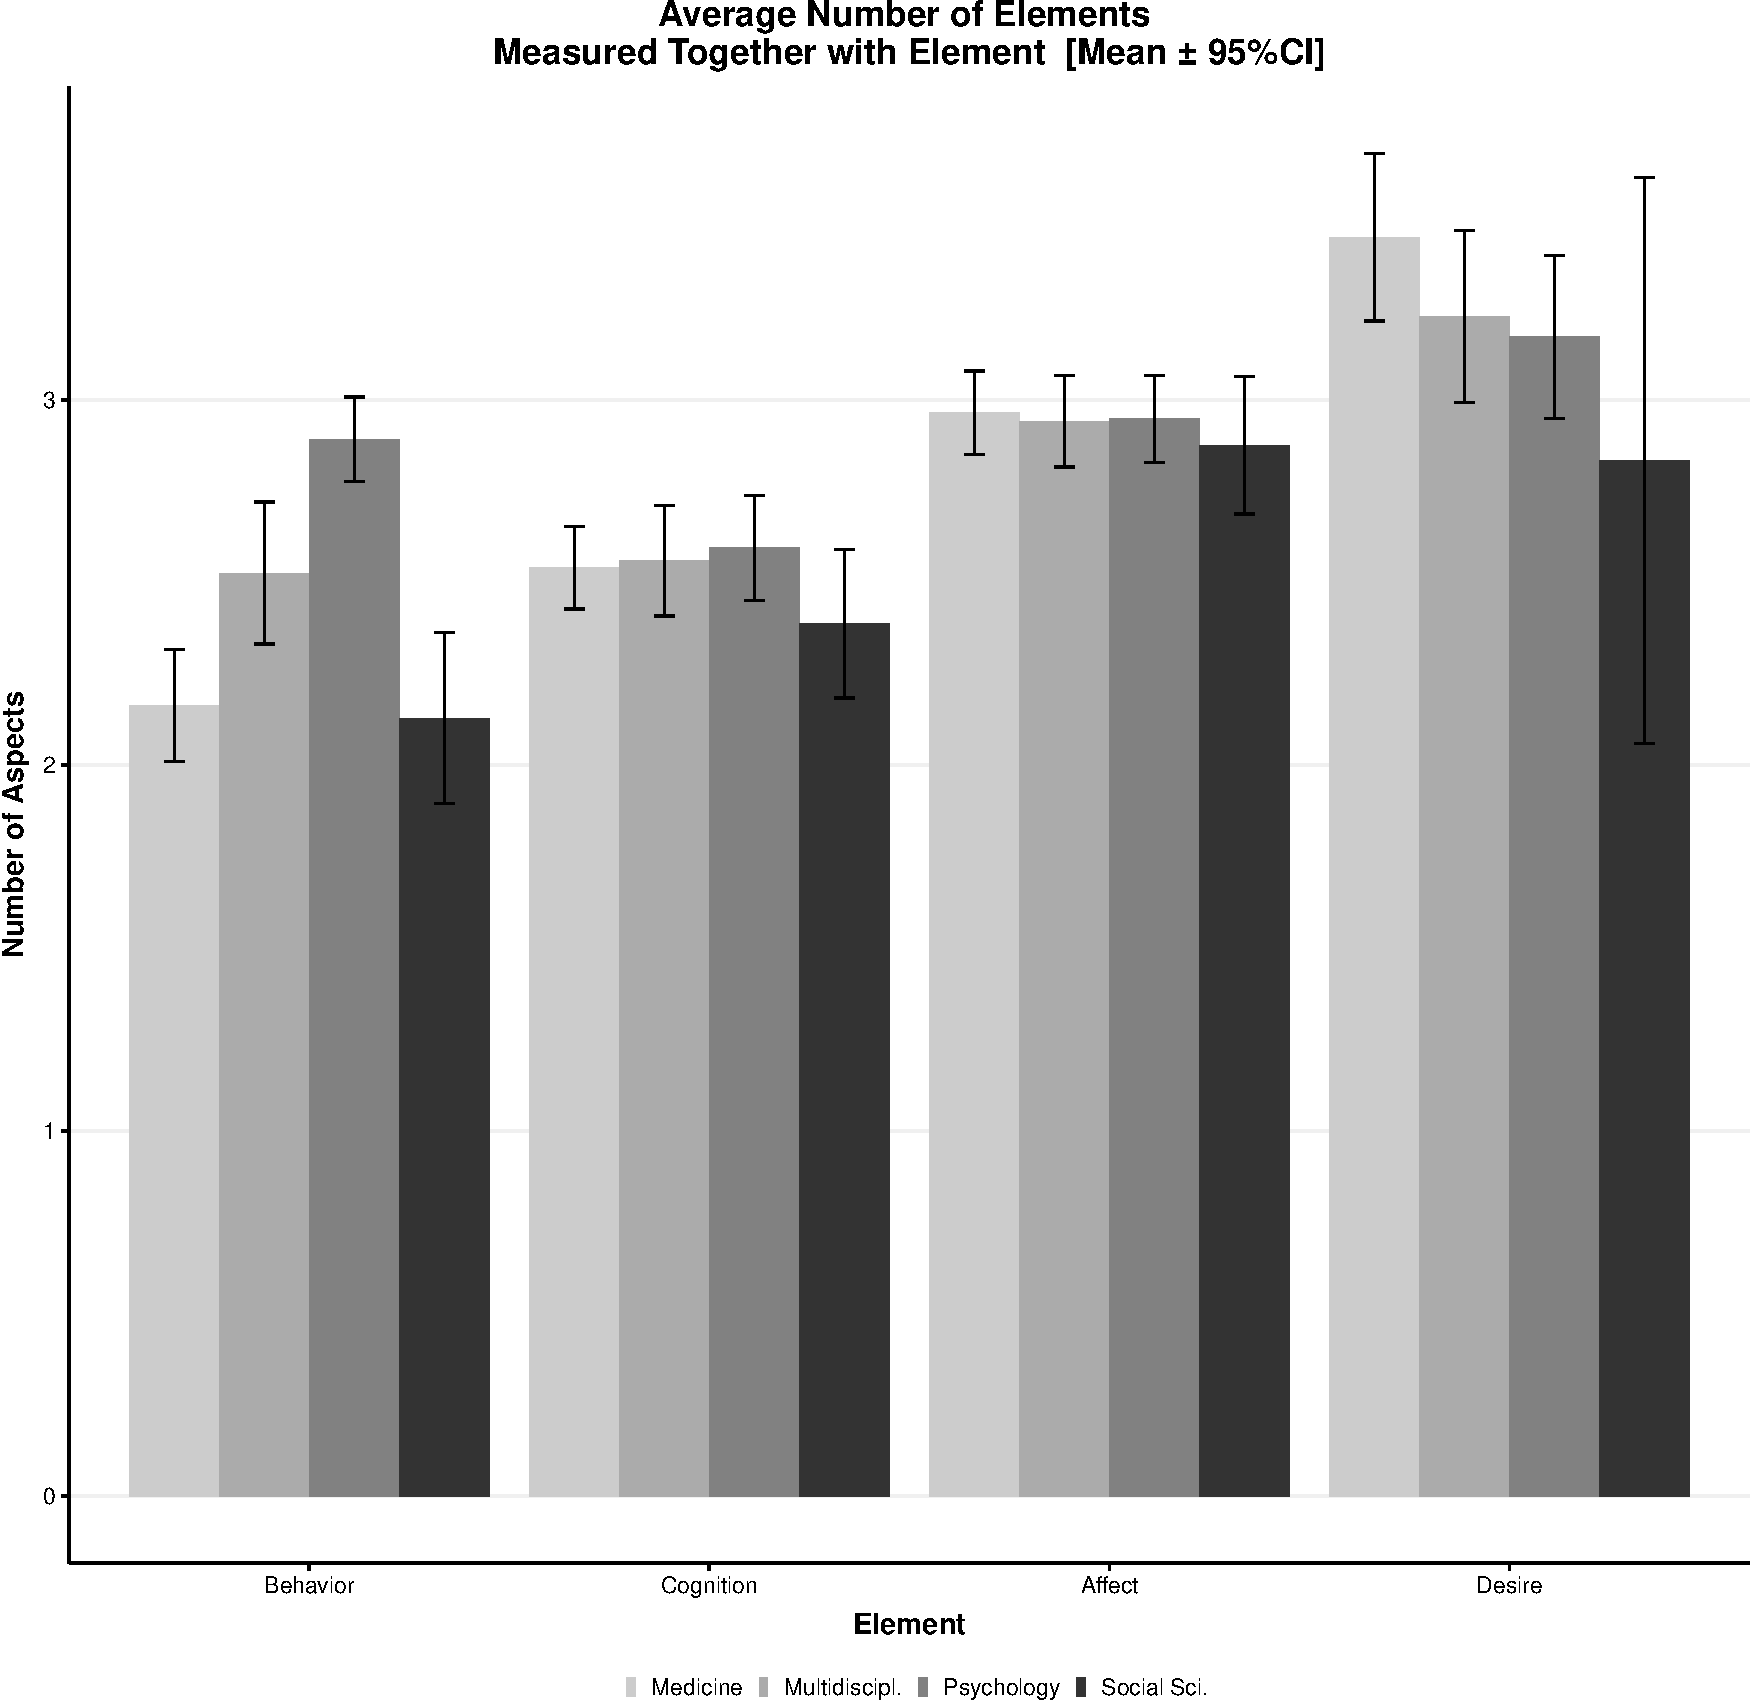
\includegraphics[width=\textwidth]{Figures/FieldElementComp-1}
\caption*{Note that these categories are not mutually exclusive (and thus not independent) because scales can include multiple experience aspects (i.e., higher complexity).}
\label{fig:FieldElementComp}
\end{figure}


\section{Discussion}
% Recap: Problem, Aim, Proposal
% Problem:
An enormous variety of aspects of our lives are affected by cultures, the psychological changes we experience when we get into continuous first-hand contact with another culture (i.e., psychological acculturation) are consequently equally plentiful and diverse.
% Aim:
In order to make sense of past theories and measures of psychological acculturation and to develop new theories and measures, it is thus necessary to build a conceptual framework that allows us to analyze, compare, and understand the individual aspects of psychological acculturation.
% Proposal:
In this paper, we have proposed that taking the fundamental aspects of the human experience (affect, behavior, cognition, and desire) would offer a comprehensive and theory-based structure to the psychological acculturation concept (in both theory and application). 

% Focus Group Discussion:
Our investigation has utilized a variety of empirical sources and applications that offer support for the applicability of an experience framework in the acculturation field. Firstly, the ABCD experience framework is, in part, based on a qualitative investigation, where key societal stakeholders have distinguished behavior, cognition, affect, and desire as important aspect of acculturation. The discussants highlighted that behavioral and cognitive aspects have more expectations from host population and are more visible, but affect and desire are equally important and often form powerful motors of change. The discussion of psychological acculturation in the field has thus offered a strong bottom-up source for the validity of the framework and the importance of all four aspects.

% Literature Review:
% Scales, Empirical, Theories
And secondly, we also applied the experience-based framework in a systematic review of past theoretical, methodological, and empirical literature on psychological acculturation. We find that all three bodies of literature focus more readily on the more external aspects of behaviors and cognitions, and less on more internal affects and desires. However, we also see that motivations (i.e., desires) play a more prominent role in the theoretical literature and interest decreases with more applied research (also see Figure \ref{fig:LiteratureComparison} A). Looking at the combinations of different experience aspects we find that across all three bodies of literature a combination of two or three aspects is most common (often including behaviors or cognitions). However, we also find that single aspect conceptualizations are substantially more common in the more applied empirical works, whereas conceptualizations that include all four experience aspects are substantially more common in the more abstract theoretical literature (also see Figure \ref{fig:LiteratureComparison} B). As a result, we also see that the most undervalued aspects often are considered in works that have already included a larger number of other aspects (also see Figure 
\ref{fig:LiteratureComparison} C). 

As a consequence, we thus find that the experience framework showed a number of useful features, which address past conceptual issues. Firstly, the experience approach is based on basic human faculties, where generally speaking every healthy person has the capacity for feelings, thoughts, desires, and behaviors. Focusing on fundamental faculties relevant to any conscious person makes the framework widely applicable across cultural contexts. ABCD frameworks have, for example, been found across cultures \citep[e.g.,][]{Bhawuk2011}\footnote{It is important to note that while anyone will have motives, emotions, thoughts, and behaviors, what one needs (e.g., belongingness or independence), feels (e.g., sadness or happiness), thinks (e.g., identification or disinterest), or does (e.g., studying or working) is highly ideographic. It is this ideographic content that makes the framework relevant to such a broad range of migration contexts. Yet, it is the content-free structure --- the presence or absence of the basic elements in conceptualizations of acculturation --- that is transferable across contexts and studies, enabling comparisons and broader conceptual discussion. It should also be noted that in our opinion such a framework does not stand in conflict with cultural or indigenous psychological concerns of an absolutist, or deterministic psychology \citep[e.g.,][]{Kim2006a}. In fact, cultural psychologists, together with many decolonial researchers, have long argued that the individual embedded and lived experience should gain a more central role in our theoretical developments \citep[e.g., ontological turn;][]{Pedersen2020}.}. It is thus not surprising that we were able to identify ABCD aspects in acculturation research from more than 40 cultural contexts (see Supplementary Information C).

Secondly, because affect, behavior, cognition, and desire broadly capture the human experience, the experience framework comprehensively captures the psychological element of acculturation. The framework, thus, captures a broad and complex phenomenon while still offering a clear and theory-driven structure of the concept and its applications. This meant that in our application very few studies did not capture any experience aspect and we were arguably able to make meaningful comparison across a wide variety of contexts and even fields.

Thirdly, experiences are also relevant across time scales. In most cases, past experiences collectively generate the present experience \citep[also see][]{Husserl1959, Heidegger1867}. As such, experiences are scale-able evaluations --- of a single situation, a recent period, or a life-long journey \citep[e.g.,][]{Clewett2019}. There is usually a clear `temporality' to human experiences and experiences can focus on the past, present, and even the future. We see this in the systematic review, where the framework was able to capture cross-sectional as well as longitudinal studies and was relevant with samples prior and post the migration event (including, prospective migrants). 

Finally, the experience conceptualization of psychological acculturation is inherently a bottom-up approach to the topic. Taking migration experiences as the starting point highlights the considerations for the lived realities of the researched individuals and communities. Scholars in the traditions of critical research methods have long highlighted the importance of including the participants in the research conceptualization process \citep[e.g.,][]{Kovach2009}. If one uses the experiences of the researched individuals to guide the study questions and design, one inevitably emphasizes the agency and needs of the community --- lending relevance and ownership of knowledge to the community \citep[e.g., ][]{Schmidt2021}. This was also one of the main focus points of the focus group discussion and was visible in the theoretical literature, that relied heavily on migration experiences and narratives to develop their theoretical works.

\subsection{Limitations}
Yet, the framework and this study are not without limitations. Notably, the framework exclusively focuses on the psychological acculturation process. This has been the explicit focus of our efforts but this also means that non-psychological aspects such as biological, cultural, or societal changes are not captured directly but only to the extent to which they impact the experiences of the involved people. Future work might want to integrate these different levels of group and individual, body and mind \citep[e.g.,][]{Eronen2021}. 

Another point that we have thus far mostly ignored is the role of the migration context. While we have argued that the framework structure (i.e., the four experience aspects) is relevant across any context, the lived experiences are often fundamentally influenced by their context and environment. Three major contextual factors often found within the literature are the cultures of the dominant and non-dominant groups, the interacting individuals, and the interaction situation or life domain. All of these contextual elements will likely have a profound impact on the experience of affects, behaviors, cognitions, and desires. Cultural differences, such as laws or norms, individual differences, such as personality or age, but also situational differences in how public or private the acculturation experience is are all likely intermingled with the individual experience aspects. This means that especially within more applied research projects such contextual considerations will be meaningful predictors of individual and group differences (for a first discussion of these contextual factors within our systematic review, see Supplemental Material C). 

\subsection{Implications}
From both the development of the experience framework of psychological acculturation and its application in the systematic review, we can thus formulate a number of lessons learned that could guide future work in the field (also see Table \ref{tab:SummaryTbl}). We believe that these have a number of broader implications for practitioners and researchers. 

%% Use of the framework:
\paragraph{Practice} The framework might be of interest to practitioners and policy-makers because it is theory-based and brings together a wide range of past literature. The structured approach might be useful in making clear and informed decisions while still considering the concept in its personal complexity. When considering psychological acculturation practitioners can choose to assess or address emotions and moods (affective acculturation), behaviors and mannerisms (behavioral acculturation), thoughts and cognitions (cognitive acculturation) or needs and desires (motivational acculturation). Whichever selection is made for an application, the framework offers a concise decision making tool and the review suggests that most theories of acculturation call for a large number of aspects.

Moreover, the research grew out of a grass-roots initiative and the personal experience framework places the individual back at the center of attention. Using the individual experience as our conceptual foundation reminds us that in clinical and social protection contexts the recipients are human beings with complex experiences. In its application, the four experience aspects thus offer a structure for building humane interventions as well as monitoring and evaluations efforts of such interventions. 

\paragraph{Research} For advancing future research projects, the systematic review and the conceptual framework can offer future perspectives for (1) the clarity of conceptualizations, (2) future empirical tests, and (3) new theoretical predictions. 

% Transfer-ability and comparability: 
% - Additionally, we observed a number of transparency and clarity issues during our systematic review: focus of aspect, operationalization (e.g., items or clear descriptions)
% - Lastly, potential data issues: broad category of migrants considered (e.g., Asian, Spanish-speaking), use of ad-hoc and non-validated scales, focus on clinical outcomes with non-clinical samples.
Our systematic review highlighted a number of transparency- and transferability issues within the field. In some works the conceptualization and operationalizations of acculturation remained vague and unexplained. Future research should clearly define which experience aspect is focused on and why a particular aspect is (ir)relevant to a specific project. Also more broadly, future research should assess the impact and transfer-ability of sample and measurement decisions, such as recruiting broad categories of migrants (e.g., "Asian", "Spanish-speaking"), the use of ad-hoc and non-validated scales, or the focus on clinical outcomes with non-clinical samples --- all of which were common within the empirical literature.

% Empirical studies:
% - re-iterate the importance of process focus (disconnect theory and empirical)
% - test theories in complexity (disconnect theory and empirical)
% - empirical studies need to investigate affect and desire are needed (highlighted in theories and focus group)
Furthermore, we find that theoretical works commonly focus on acculturation as a process that includes multiple experience aspects, while empirical works were considerably more static and narrow in their conceptualization. Future research should, thus, consider more longitudinal and multi-faceted conceptualizations of acculturation to meaningfully test theoretical models and -predictions in their entirety. A similar gap exists in the focus on specific aspects, where affect and desire conceptualizations are highlighted in theoretical works as well as our qualitative study but remain relatively absent in empirical works. Future empirical studies will thus need to investigate the mechanisms and roles of affective and motivational acculturation.

% Relationships:
% - need to investigate the relationships between different experience aspects. 
% - need to investigate the relationships of experience aspects with other concepts.
Finally, our framework also opens up the possibility to investigate relationships between individual experience aspects of acculturation and of these aspects with other concepts. Future research could, for example, assess whether a certain aspect precedes another or how one aspect might feed back into another (e.g., motivations guiding cognition and affect, which in turn drive behavior. cf., theory of reasoned goal pursuit; \citealp{Ajzen2019}). Similarly, the subdivision in experience aspects also allows for more nuanced investigations of these acculturation aspects to other concepts (e.g., does behavioral acculturation have the same impact on health as emotional acculturation?). And in its broadest implication, the four experience aspects might aid in future integrations of the more than 90 mostly independent theoretical works and the even larger body of methodological and empirical applications \citep[e.g.,][]{Maertz2016}. 

\begin{table}%[hbt]
\caption{Synthesis Summary and Future Perspectives.}
\label{tab:SummaryTbl} 

\footnotesize

\begin{tabular}{>{\raggedright\arraybackslash}p{0.50\linewidth} 
>{\raggedright\arraybackslash}p{0.50\linewidth}}

\hline 
Critical issues identified in systematic review &
Perspective / Suggestions \\ 
\hline

\vspace{-0.5em} \hangindent=0.55cm 1.~ Theoretical and empirical conceptualizations of psychological acculturation have been diverse and unstructured.  & 
\vspace{-0.5em} The affect, behavior, cognition, desire distinctions could be used to structure acculturation conceptualizations. \\ 

\vspace{-0.5em} \hangindent=0.55cm 2.~ Empirical studies focus on cross-sectional outcome conceptualizations while theories predominantly conceptualize psychological acculturation as a process. & 
\vspace{-0.5em} In empirical works a stronger focus on longitudinal acculturation assessments is needed to congruently test theories empirically. \\ 

\vspace{-0.5em} \hangindent=0.55cm 3.~ Theories include substantially more experience aspects in their conceptualization than empirical studies. & 
\vspace{-0.5em} Empirically, investigations of more acculturation aspects are needed to congruently test theories empirically. \\ 

\vspace{-0.5em} \hangindent=0.55cm 4.~ There has been little empirical focus on emotional and motivational aspects, even though they are important in theories and qualitative discussions. & 
\vspace{-0.5em} To close this gap, empirical studies that investigate the internal aspects of affect and desire are needed. \\ 

\vspace{-0.5em} \hangindent=0.55cm 5.~ The choice of investigated acculturation aspects have often remained elusive in methodological and applied empirical literature. & 
\vspace{-0.5em} For replications, comparisons, and theoretical synthesis, research and intervention choices need to be transparent. Which aspect is focused on? Why is an aspect (ir)relevant to the project? \\ 

\vspace{-0.5em} \hangindent=0.55cm 6.~ Operationalizations and measurements of acculturation have often remained unclear (especially with ad-hoc measures or non-validated modifications and non-disclosed items). & 
\vspace{-0.5em} As long as the field faces conceptual issues, transparency in measurement would be important. Either items or clear content descriptions should be available. And research should assess the impact of non-validated scales.\\ 

\vspace{-0.5em} \hangindent=0.55cm 7.~ In theoretical and empirical work, experience aspects are commonly considered independently. & 
\vspace{-0.5em} There is a need to investigate the relationships between different experience aspects. \\ 

\vspace{-0.5em} \hangindent=0.55cm 8.~ Theories have independently been applied to different aspects (e.g., behavioral or cognitive orientations), but effects have rarely been compared across aspects.  & 
\vspace{-0.5em} To synthesize past research, relationships of acculturation with other concepts need to be compared where acculturation has been conceptualized within different experience aspects. \\ 

\vspace{-0.5em} \hangindent=0.55cm 9.~ Psychological and cultural adaptation (as a form of acculturation) have often been conceptualized inconsistently. & 
\vspace{-0.5em} Future investigations and interventions could consider functionality and adaptation within each experience aspect. \\ 

\vspace{-0.5em} \hangindent=0.65cm 10. The normative aim of acculturation conceptualizations are often unclear (e.g., does the conceptualization aim to benefit an individual or society?). & 
\vspace{-0.5em} There is a need to discuss the normative expectations of acculturation conceptualizations within empirical and theoretical work \citep[e.g.,][]{Ager2008a}. \textit{Maybe move to conceptualization (point 5)?} \\ 

\vspace{-0.5em} \hangindent=0.65cm 11. The non-dominant target group has often been defined very broadly (e.g., any migrant, Asia, Spanish-speaking, third world). & 
\vspace{-0.5em} Research questions, conceptualizations, and measurements concerning acculturation should be specific to all considered cultural contexts or should be transferable across all considered cultural contexts. \\ 

\vspace{-0.5em} \hangindent=0.65cm 12. We identified \nTheo\ (mostly independent) theoretical works. & 
\vspace{-0.5em} Future research should assess the possibility of theoretical synthesis. The experience framework might offer a conceptual lens for such a synthesis.\\ 

\vspace{-0.5em} \hangindent=0.65cm 13. Acculturation measures are often validated within specific cultural contexts but are applied within other cultural contexts. & 
\vspace{-0.5em} Future research needs to investigate the potential impact of measure transference. \textit{Maybe move to measurement (point 6)?} \\ 

\vspace{-0.5em} \hangindent=0.65cm 14. Empirical work has had a strong focus on clinical outcomes but utilized few clinical samples. & 
\vspace{-0.5em} \textit{probably drop this.} \\ 

\hline

\end{tabular}
\end{table}


In sum, a framework for psychological acculturation based on core aspects of experiences might thus offer a useful tool for both researchers and practitioners. The framework offers a theory-based way of comprehensively assessing, comparing, and understanding acculturation. We bring together insights from experts in the field as well as a wide array of past advances in the literature.

%\newpage

\printbibliography

\appendix

\section{Search Strategy}
\label{app:AppendixSearchStrategy}

To assess the past empirical and theoretical literature on psychological acculturation, we performed a systematic review. We first read seminal and review works within the field \citep[including,][]{Ward2019, Berry1997b, Berry2003, Szapocznik1978, Sam2006a, Rudmin2003a}. Based on our reading of the literature, we designed a comprehensive literature search strategy in an iterative fashion. 

For the empirical work on acculturation, we performed a literature search on March 4\textsuperscript{th}, 2020 and February 14\textsuperscript{th}, 2021, within the ``APA PsycINFO'' bibliographic databases using the EBSCO\textit{host} provider. The databases also included the PsycARTICLES, PsycBOOKS, and PsycCRITIQUES databases as well ProQuest Dissertations with psychological relevance. The second literature search included alternate terms used less frequently to describe what we mean with psychological acculturation, including "transculturation" and "cultural transition". Additionally, the second search removed limiter terms that could have exclude interdisciplinary investigations and focused on human participants.

For the theoretical literature performed an additional, more specific, search of the same databases as well as the Web of Science Core Collection using the Clarivate Analytics provider on March 3\textsuperscript{rd}, 2021.

In designing our search strategy we used an adapted version of the `SPIDER' research tool \citep[e.g.,][]{Cooke2012}. We utilized the \textit{Evaluation} element mainly to exclude articles that were not relevant to the search. The exact search terms used are listed in Table \ref{tab:SearchStrategiesTab} below.

\begin{table}
\caption{Search Strategy Cultural Adaptation Review}
\label{tab:SearchStrategiesTab} 
\begin{tabular}{ll}
\hline
Element & Search Terms \\ 
\hline \\ [-0.5em]

% Sample
Sample & 
    (Immigration OR migration OR migrant OR immigration OR refugee) \\ 
    \\ [-0.25em]
    
% Phenomenon of Interest
\begin{tabular}[t]{@{}l@{}}Phenomenon \\of Interest\end{tabular} & 
    \begin{tabular}[t]{@{}l@{}}(acculturation OR enculturation OR transculturation OR \\
    assimilation OR "social integration" OR "cultural adaptation" OR \\
    "cultural adjustment" OR "cultural transition")\end{tabular}  \\ 
    \\ [-0.25em]
    
% Design
Design & 
    \begin{tabular}[t]{@{}l@{}}("measurement tool" OR scale OR instrument OR \\
    questionnaire OR survey OR definition OR inventory)\end{tabular}  \\ 
    \\ [-0.25em]
    
% Evaluation
Evaluation & 
    \begin{tabular}[t]{@{}l@{}}NOT (parent* OR college OR resilience OR treatment OR \\
    intervention OR therapy)\end{tabular}  \\ 
    \\ [-0.25em]
    
% Research Type
Research type * & 
    (quantitative OR qualitative OR "mixed method") \\ [0.75em] 
    \hline

% Note
\multicolumn{2}{l}{* This element was ultimately dropped because it was too sensitive in PsycInfo.}
\end{tabular}
\end{table}


\end{document}

%% 
%% Copyright (C) 2019 by Daniel A. Weiss <daniel.weiss.led at gmail.com>
%% 
%% This work may be distributed and/or modified under the
%% conditions of the LaTeX Project Public License (LPPL), either
%% version 1.3c of this license or (at your option) any later
%% version.  The latest version of this license is in the file:
%% 
%% http://www.latex-project.org/lppl.txt
%% 
%% Users may freely modify these files without permission, as long as the
%% copyright line and this statement are maintained intact.
%% 
%% This work is not endorsed by, affiliated with, or probably even known
%% by, the American Psychological Association.
%% 
%% This work is "maintained" (as per LPPL maintenance status) by
%% Daniel A. Weiss.
%% 
%% This work consists of the file  apa7.dtx
%% and the derived files           apa7.ins,
%%                                 apa7.cls,
%%                                 apa7.pdf,
%%                                 README,
%%                                 APA7american.txt,
%%                                 APA7british.txt,
%%                                 APA7dutch.txt,
%%                                 APA7english.txt,
%%                                 APA7german.txt,
%%                                 APA7ngerman.txt,
%%                                 APA7greek.txt,
%%                                 APA7czech.txt,
%%                                 APA7turkish.txt,
%%                                 APA7endfloat.cfg,
%%                                 Figure1.pdf,
%%                                 shortsample.tex,
%%                                 longsample.tex, and
%%                                 bibliography.bib.
%% 
%%
%% End of file `./samples/longsample.tex'.
